\documentclass[10pt,twoside]{amsart}
\usepackage{avinash}
% -----------------------------------------------------------------------------------------
\title[Submodular Knapsacks : A Discussion]{%
submodular knapsacks : a discussion \\[1.75em]}
\author{Avinash Bhardwaj}

% -----------------------------------------------------------------------------------------
\begin{document}
\onehalfspacing

%\BCOLHeader
%
%\funding[Grant $\#$ AFORS FA9550-10-1-0168 from the US Department of Defense.]
%
%\affiliation{A. Atamt\"{u}rk}{Industrial Engineering and Operations Research, University of California, Berkeley, CA $94709-1777$\,\,\Letter\,\,\texttt{\href{mailto:atamturk@berkeley.edu}{atamturk@berkeley.edu}}}
%\affiliation{A. Bhardwaj}{Industrial Engineering and Operations Research, University of California, Berkeley, CA $94709-1777$\,\,\Letter\,\,\texttt{\href{mailto:avinash@ieor.berkeley.edu}{avinash@ieor.berkeley.edu}}}

\date{}
\maketitle

\begin{abstract}
    \vspace{2.25em} In the following discussion we study the facial structure of the convex hull of the level sets of a given submodular set function $f: \binset^n\mapsto \R$. In particular we derive valid inequalities and their extensions for the general lower level sets of submodular set functions, and propose the facet defining conditions for the same. The following discussion is novel in sense that it relaxes the monotonicity assumptions made in earlier studies and thus offers a generalization to earlier studies on this subject matter. We will follow a bottom up hierarchical structure to derive the appropriate expressions for the valid inequalities and their extensions from the linear knapsack inequalities corresponding to the extended polymatroid of the set function in context.
\end{abstract}

\singlespacing
\section{Introduction}
Given a finite ground set $N$, a set function $f\,:\,2^N\,\rightarrow {\R}$ is supermodular on $N$ if
\begin{align*}
    f(S) + f(T) \leq f(S\cup T) + f(S\cap T)\,\,\,\forall\,S,T\,\subseteq N.
\end{align*}
Throughout, by an abuse of notation we, refer to a set function also as $f(\mathcal{X}_S)$, where $\mathcal{X}_S$ denotes the binary characteristic vector of $S\subseteq N$.

For notational simplicity, we denote a singleton set $\{i\}$ with its unique element $i$. For a vector $\v \in {\R}^N$, we use $\v(S)$ to denote $\sum_{i\inset S}\,v_i$ for $S\subseteq N$. Given a set function $f$ on $N$ and $i \in N$, denote the difference function with respect to the set function $f$ as,
\begin{align*}
    \rho_i(S) := f(S\cup i) - f(S) \,\,\,\text{for $S \subseteq N\setminus i$}
\end{align*}
Observe that $f$ is supermodular if and only if $\rho_i(S) \leq \rho_i(T)\,\forall\,S\subseteq T\subseteq N\setminus i$ and $i \in N$; that is the difference function $\rho_i$ is non-decreasing on $N\setminus i$ (Schrijver, \cite{Schrijver2003}).

\subsection{Motivation}
\subsubsection{Chance Constraints with Uncertain Coefficients}\hfill

Our prime motivation to study knapsack sets with submodular set functions stems from the need to analyze linear $0-1$ covering constraints with uncertain coefficients. For example, consider the following covering constraint,
\begin{align}
\label{cons:covering}
    \boldsymbol{\xi}'\x \geq d
\end{align}
where $\xi_i$, $i \in \{1,2,\ldots, N\}$ are random with a support $\Xi$. Constraint \eqref{cons:covering} does not define a deterministic feasible set. In a deterministic realm we can approximate the above covering constraint by the following probabilistic constraint,
\begin{align}
\label{eq:chanceconstraint}
    \text{\bf{Pr}}(\boldsymbol{\xi}'\x \geq d) \geq 1 - \epsilon,\,\,\,\,\epsilon > 0.
\end{align}

For $x\inset \{0,1\}^N$, Charnes and Cooper \cite{Charnes1963} suggest under \textit{nominal} conditions that Constraints of type \eqref{eq:chanceconstraint} (or approximations thereof) can be modeled as conic-quadratic $0-1$ constraints,
\begin{align}
\label{eq:equivalence}
  X_{CQ} := \set{\x\inset \{0, 1\}^m}{\mathbf{u}^T\x - \Omega(\epsilon)\norm{\mathbf{\Sigma}^{\frac{1}{2}}\,\x}\, \geq\, d}
\end{align}
where $u_e$ is the nominal value, $\boldsymbol\Sigma$ is the covariance matrix, and $\Omega(\epsilon) > 0$ is the scaling factor. The term $\Omega(\epsilon)\norm{\mathbf{\Sigma}\,\x}$ is used to build sufficient slack into the constraint to accommodate the variability of $\xi_i$ around the nominal value $u_i$. If $\xi_i$'s are normally distributed independent random variables, then letting $u_i$ and $\sigma_{ii}$ be the mean and standard deviation of $\xi_i$, $0 \leq i \leq m$, and $\Omega(\epsilon) = -\phi^{-1}(\epsilon)$ with $0 < \epsilon < 0.5$, where $\phi$ is the standard normal cumulative distribution function, the set of $0-1$ solutions for the probabilistic covering constraint \eqref{eq:chanceconstraint} is exactly $X_{CQ}$. On the other hand, if $\xi_i$'s are known only through their first two moments $u_i$ and $\sigma^2_{ii}$, then any point in $X_{CQ}$ with $\Omega(\epsilon) = \sqrt{(1-\epsilon)/\epsilon}$ satisfies the probabilistic constraint \eqref{eq:chanceconstraint} \cite{Bertsimas2005,Ghaoui2003}. Alternatively, if $\xi_i$'s are only known to be symmetric with support $[u_i - \sigma_{ii}, u_i + \sigma_{ii}]$, then points in $X_{CQ}$ with $\Omega(\epsilon) = \sqrt{\ln(1/\epsilon)}$ satisfy constraint \eqref{eq:chanceconstraint} \cite{Ben-Tal2000,Ben-Tal2002}. Hence, under different assumptions of uncertainty on $\boldsymbol{\xi}$, one arrives at different instances of the conic quadratic knapsack set $X_{CQ}$.\\

Consider now a set function $f : 2^N \rightarrow R$ defined as,
\begin{align}
\label{function:f}
	f(S) = \mathbf{u}(S) + g(\mathbf{c}(S)),
\end{align}

where $g$ is a concave function and $\mathbf{u}(S)$ and $\mathbf{c}(S)$ denote the sums of the components of $\mathbf{u}, \mathbf{c}\inset {\R}^N$ on $S\subseteq N$. Ahmed and Atamt\"{u}rk \cite{Ahmed2011} show that if $\mathbf{c} > 0$, then $f$ is submodular on $N$. Observe that, in case $\xi_i$'s are uncorrelated, $X_{CQ}$ is a special case of $X$, observe that the conic quadratic constraint defining $X_{CQ}$ can be written as
\begin{align}
\label{ineq:functionform}
	-\mathbf{u}^T\x + \Omega\norm{\mathbf{\Sigma}^{\frac{1}{2}}\,\x}\, \leq\, - d
\end{align}

Because $\x$ is a binary vector, letting $c_i = \Omega^2 \sigma^2_i$ for $i\inset N$, we see that $\mathcal{X}_S$,  $S \subseteq N$ is feasible for \eqref{ineq:functionform} if and only if $S$ satisfies,

\begin{align}
	f(S) =  -\mathbf{u}(S) + \sqrt{\mathbf{c}(S)} \leq -d
\end{align}

The majority of the research on the nonlinear knapsack problem is devoted to the case with separable nonlinear functions \cite{Morin1976}. Hochbaum \cite{Hochbaum1995} maximize a separable concave objective function, subject to a single ``packing'' constraint. They prove that the although seemingly more difficult in comparison with the linear knapsack, the complexity of the non-linear knapsack is similar. There are few studies on the nonseparable knapsack problem, most notably on the knapsack problem with quadratic objective and linear constraint. Helmberg et al. \cite{Helmberg2000} give semidefinite programming relaxations of knapsack problems with quadratic objective. Ahmed and Atamt\"{u}rk \cite{Ahmed2011} consider maximizing a submodular function over a linear knapsack constraint. Atamt\"{u}rk and Narayanan \cite{Atamturk2010} describe a general mixed-integer rounding for conic quadratic mixed integer sets. \c{C}ezik and Iyengar \cite{Cezik2005} study techniques for generating valid convex constraints for mixed 0-1 conic programs and show that many of the techniques developed for generating linear cuts for mixed 0-1 linear programs, such as the Gomory cuts, the lift-and-project cuts, and cuts from other hierarchies of tighter relaxations, extend in a straightforward manner to mixed 0-1 conic programs. These approaches although efficient, are generic, and do not exploit any special structure(s) associated with the problem. We refer the reader to \cite{Bretthauer2002,Kellerer2004} for a survey of nonlinear knapsack problems. The literature is scarce in case of knapsack sets associated with set functions. Assume $f$ to be a given submodular set function on a finite set $N$. The lower level set of $f$, $K_f \define \set{\x\inset \binset^n}{f(\x) \leq b}$, $b \in \R^n$ in case when $f$ is non-decreasing on $N$ was recently studied by \atam and Narayanan \cite{Atamturk2009333}. Alternatively, when $f$ is non-increasing as discussed above, the facial structure has been studied by \atam and Bhardwaj in form of pack inequalities and their extensions. The most recent study on quadratically constrained knapsacks is by \atam et al. \cite{Atamturk2013} where they study the extensions and separation of cover inequalities for conic quadratic knapsack constraints with generalized upper bounds.

It is of interest to study the polyhedral structure of this level set when the monotonicity assumptions are relaxed. An additional application lies in form of the following second order cone set, $$S_{\text{SOC}} \define \set{\x \in \binset^n}{\mathbf{a}'\x - \Omega\sqrt{\x'\Sigma\x}\geq b},$$ $\Sigma = \lbrack\sigma_{ij}\rbrack_{1\leq i, j \leq n}\succeq 0,\,\, a_i \geq \Omega\cdot\sigma_i\,\forall\, 1\leq i \leq n$. This is the inner approximation of the chance constraint \eqref{eq:chanceconstraint} when $\xi_i,\,\,i\in N$ are correlated.\\

It can be seen $S_{\text{SOC}} = S_{\text{QP}} \cap \set{x\in \binset}{\a'\x \geq b}$, where,
$$
        S_{\text{QP}} \define \set{\x \in \binset^n}{\sum_i{\alpha_ix_i + 2\sum_{j>i}{\beta_{ij}x_ix_j}} \leq \gamma}
$$
and $\alpha_i = (2a_ib + \Omega^2\sigma_{ii}^2 - a_i^2)$, $\beta_{ij} = -(a_ia_j - \Omega^2\sigma_{ij}) \leq (\Omega^2\sigma_{i}\sigma_j- a_ia_j) \leq 0$ and $\gamma = b^2$.

\begin{prop}
  \label{prop:Qsubmod}
  Consider a set function $f: \binset^n\mapsto \R$, defined as a binary quadratic mapping,
  \begin{align}
    f(\x) \define \x'\,Q\,x
  \end{align}
  where $Q$ is a $n\times n$ off-diagonal matrix. $f(\cdot)$ is submodular if and only if $$Q_{ij} \leq 0,\,\, 1\leq \,i,\,j\,\leq n.$$
\end{prop}
\begin{proof}
  Consider,  $S\subseteq T \subseteq N\sm i\,\,\,\,\,\,\,$ for some $i \inset N$
  Now,
  \begin{align*}
    \rho_i(T) - \rho_i(S) & = f(T\cup i) - f(S\cup i) - f(T) + f(S)\\
                        & = Q_{i(j\in T)} - Q_{i(j\in S)}\\
                        & = Q_{i(j\in T\sm S)}\\
                        & \leq 0
  \end{align*}
  where the last inequality follows from non-positivity of $Q_{ij} \leq 0,\,\, 1\leq \,i,\,j\,\leq n$. Thus, we have $\rho_i(S) \leq \rho_i(T)\,\,$ $\forall\,\,S\subseteq T \subseteq N\sm i\,\,\,\,\,\,\,$ $i \inset N$ proving submodularity of $f(\cdot)$.

  Alternatively, assume $f(\cdot)$ is submodular, thus $\forall\,\,S\subseteq T \subseteq N\sm i\,\,\,\,\,\,\,$ $i \inset N$,
  \begin{align*}
    0 \leq & \, \rho_i(S) - \rho_i(T)\\
    0 \leq & \, f(S\cup i) - f(T\cup i) - f(S) + f(T)\\
    0 \leq & \, Q_{i(j\in S)} - Q_{i(j\in T)}\\
    0 \geq & \, Q_{i(j\in T\sm S)}
  \end{align*}
  Thus, $Q_{i(j\in T\sm S)} \leq 0$, $\forall\,\,S\subseteq T \subseteq N\sm i\,\,\,\,\,\,\,$ $i \inset N$, which yields $Q_{ij} \leq 0,\,\, 1\leq \,i,\,j\,\leq n.$
\end{proof}

\begin{cor}
  \label{cor:Qsubmod}
  Consider a set function $f: \binset^n\mapsto \R$, defined as a binary quadratic mapping,
  \begin{align}
    f(\x) \define \a'x + \x'\,Q\,x
  \end{align}
  where $Q$ is a $n\times n$ matrix and $\a \in \R$. $f(\cdot)$ is submodular if and only if $$Q_{ij} \leq 0,\,\, 1\leq \,i,\,j\,\leq n\,,\,i\neq j.$$
\end{cor}

Proposition \ref{prop:Qsubmod} and Corollary \ref{cor:Qsubmod} in effect suggest that $S_{\text{QP}}$ is the lower level set of a submodular set function. The associated set however is not necessarily monotone. A requirement to study the polyhedral structure of the level sets associated with the generic submodular set functions is thus apparent. Albeit the motivation stems from the submodular quadratic maps, the following discussion is valid for knapsack sets associated with submodular functions in general.

\section{Linear $0-1$ Knapsack Set}
The knapsack problem is one of the most celebrated problems in optimization literature. Most of the literature available on the knapsack problem is for the linear knapsack set (binary, integer, mixed-integer). The polyhedral analysis of the linear knapsack set was initiated by Balas \cite{Balas1975,Balas1978}, Hammer et al. \cite{Hammer1975}, and Wolsey \cite{Wolsey1975}. For an extensive review of theoretical and computational results on linear knapsacks we refer the reader to \cite{Atamturk2003,Atamturk2005,Gu1998,Martello1990}. In this section we'll review the results and literature for the case of linear $0-1$ knapsack set $K \define \set{\x \in \binset^n}{\mathbf{a}\x \leq b},$ $\mathbf{a} \geq 0$.

In the following, we review some of the results on the valid inequalities for $\conv(K)$
\begin{prop}
  Inequality $x_i \geq 0$, $i\in N$ is facet defining for $\conv(K)$.
\end{prop}

\begin{prop}
  Inequality $x_i \leq 1$, $i\in N$ is facet defining for $\conv(K)$ if and only if $a_i + a_j \leq b$, $\forall\,\,j\inset N\setminus\{i\}$.
\end{prop}

\begin{prop}
  If the inequality $\boldsymbol\alpha\x \leq \beta$ defines a facet for $\conv(K)$ not including $\mathbf{0}$ then $\beta > 0$ and $\alpha_j \geq 0$, $\forall\,\,j\in N$.
\end{prop}

\subsection{Cover Inequalities}
\begin{dfn}
  A subset $C$ of the index set $N$ is called a \textit{cover} if $\lambda \define a(C) - b > 0.$
\end{dfn}

For a cover $C$, let us consider the restriction $K_C$ obtained by fixing all $x_i,\, i\inset N\setminus C$ to zero. Since the sum of the coefficients $a_i,\, i\inset C$ exceeds the knapsack capacity by $\lambda > 0$, all variables $x_i,\, i\inset C$ cannot take a value of one simultaneously for any $\x \inset K$. Therefore, the \textit{cover inequality} \cite{Balas1975,Hammer1975,Wolsey1975}
\begin{align}
        x(C) \leq |C| - 1 \label{ineq:cover}
\end{align}
is valid for $\conv(K)$. Cover inequality defines a facet for $\conv(K_C)$ if and only if $C$ is a minimal cover, that is, $\a(C\setminus \{i\}) \leq b,\,\forall\,i\inset C$.

\subsubsection{Extensions of Cover Inequalities}
\label{sec:extension}
\hfill

Extensions are a means to strengthen the inequalities based on restrictions of feasible sets, in this case the cover inequalities. For a cover $C \subseteq N$, consider the cover inequality \eqref{ineq:cover}.
\begin{align*}
        \x(C) \leq |C| - 1
\end{align*}

An important and very useful concept in deriving strong valid inequalities is lifting of inequalities. Lifting refers to extending valid inequalities for low dimensional restrictions of polyhedra to ones that are valid in high dimensions. The concept of lifting has been introduced by Gomory \cite{Gomory1969451} in the context of the group problem. Padberg \cite{Padberg75} described the sequential lifting procedure for $0-1$ programming. Since then lifting has been studied and used extensively (\atam \cite{Atamturk04}; Balas and Zemel, \cite{Balas1978}; Escudero, Gar\'{i}n, and P\'{e}res, \cite{Escudero2003211}; Gu, Nemhauser, and Savelsbergh,\cite{Gu1998,Gu1999a,Gu1999b,Gu2000}; Johnson and Padberg, \cite{Johnson198118}; Louveaux and Wolsey, \cite{Louveaux07}; Marchand and Wolsey, \cite{Marchand99}; Nemhauser and Vance, \cite{Nemhauser1994}; Padberg, \cite{Padberg73}; Richard, de Farias, and Nemhauser, \cite{JP2002}; Sherali and Lee, \cite{Sherali95}; Wolsey, \cite{Wolsey1975,Wolsey77}; Zemel, \cite{Zemel78,Zemel89}), particularly, for $0-1$ and mixed $0-1$ programming problems. We can strengthen the cover inequality by introducing the variables not present in the inequality ($x_i,\,\forall\, i \inset N\sm C$) multiplied with appropriate coefficients.  The lifted cover inequality in this case can be represented as,
\begin{align}
        \x(C) + \sum_{i\,\in N\sm C} \alpha_i x_i \leq |C| - 1 \label{ineq:liftedcover}
\end{align}
where $\alpha_i \geq 0,\,i\in N\sm C$ are the corresponding lifting coefficients. Obtaining exact lifting coefficients entails computing the lifting function $\Theta(\cdot)$ of cover inequality \eqref{ineq:cover},

\begin{align}
  \Theta(a) \define |C| - 1 - \max\set{\sum_{i\in C} x_i}{\sum_{i\in C}\, a_ix_i \leq b - a} \label{func:liftingfn}
\end{align}

for $a \geq 0$. Obtaining a closed form expression for the lifting function is not always trivial. Extensions are computationally inexpensive special cases of lifting, wherein instead of deriving the exact lifting coefficients, we identify whether a variable $x_i,\,i\in N\sm C$ can be introduced into the cover inequality with a coefficient $\alpha_i \geq 1$. Let $E$ be a set of all such indices, i.e. $E \define \set{i\inset N\sm C}{\alpha_i \geq 1}$. The extended cover inequality thus is,
\begin{align}
        \x(C\cup E) \leq |C| - 1 \label{ineq:extdcover}
\end{align}
%Consider a permutation of the indices in the complement of the cover set $C$, in particular, let $\{(1),(2),\ldots,(|N\sm C|)\}$ be the permutation of elements of the set $N\sm C$. Define $C_k \define C \cup \{(1),(2),\ldots,(k)\},\, 0\leq k\leq |N\sm C|$ with $C_0 = C$. The extension $E$ with respect to $C$ can be represented as,
%\begin{align}
%  E \define \set{(k) \in N\sm C}{a_{(k)} > \underset{j\in C_{k-1}}{\max}\, a_j - \lambda_{k-1}}
%\end{align}
%where $\lambda_k = \lambda_{k-1} - \left(\underset{j\in C_{k-1}}{\max}\, a_j - a_{(k)}\right)^+$ and $\lambda_0 = \lambda$
%
%It follows from definition that $\lambda_k > 0\,\,0\leq k \leq |N\sm C|$, which in turn yields the validity of the extended cover inequality.

% -------------------------------------- IGNORE ------------------------------------
Consider a subset of indices $\bar{E} \subseteq N\sm C$. Assume that the corresponding variables $x_i,\,i\in \bar{E}$ have been included in the extended cover inequality. Consider the variable $x_k, k \in N\sm (C\cup \bar{E})$ to be included next in the extended cover.
\begin{prop}
  $\alpha_k \geq 1,$ if $a_k > \underset{j\in C\cup \bar{E}}{\max}\, a_j - \lambda$
\end{prop}
%
%Observe however, if $C$ is a cover, we can extend the cover inequality corresponding to $C$, for all $k \in N\sm C$ if $a_k > \underset{j\in C}{\max}\, a_j - \lambda$. This can be understood as we cannot have more than $|C|-1$ $x_i,\,\,i\in C\cup \set{k \in N\sm C}{a_k > \underset{j\in C}{\max}\, a_j - \lambda}$ assigned a value of $1$. As a contradiction, define $p = \underset{j\in C}{\arg\max}\, a_j$ and $E = \set{k \in N\sm C}{a_k > a_p - \lambda}$ consider that $\sum_{i\in C\cup E} x_i \geq |C|$. Now see that since, $\sum_{i\in C} a_i > b$,
%\begin{align*}
%    \sum_{i\in C\cup E} a_ix_i & > \sum_{i\in C} a_ix_i + \sum_{j \in E} (a_p - \lambda)x_j
%\end{align*}
% -------------------------------------- IGNORE ------------------------------------

\atam \cite{Atamturk2005}, Balas and Zemmel \cite{Balas1978}, Gu et al. \cite{Gu2000} provide a characterization of the lifting function $\Theta(a)$ for the cover inequalities for $0-1$ integer knapsack set. This characterization yields a sequence independent lifting procedure, and as a special case, a sequence independent extension for the cover inequalities. Attributed to this, we can further simplify the extension procedure to a sequence independent extension.
\begin{cor}
\label{cor:ext}
  For $k\in N\sm C,$ $\alpha_k \geq 1,$ if $a_k > \underset{j\in C}{\max}\, a_j - \lambda$.
\end{cor}

The corresponding extension set $E \subseteq N\sm C$ can now be defined as,
\begin{align}
\label{set:ext}
        E \define \set{i\inset N\sm C}{a_i > \underset{j\in C}{\max}\, a_j - \lambda}
\end{align}

\begin{prop}
  The extended cover inequality \eqref{ineq:extdcover} is valid for $\conv(K)$. In addition, inequality \eqref{ineq:extdcover} defines a facet of $\conv(K_{C\cup E})$ if and only if $C$ is minimal and $\forall\, i\inset E$ $\exists\, \text{distinct }\{j,k\}\inset C$ such that $\a(C\cup \{i\}\sm \{j,k\}) \leq b$.
\end{prop}

\subsubsection{Sequence Independent Bounds for Lifting Coefficients}\hfill\label{sec:seqindp}

 As a follow up to extensions, it is of interest to understand whether the lifting coefficients $\alpha_i,\,i\in N\sm C$ in the lifted cover inequality \eqref{ineq:liftedcover} can be computed efficiently in general. Sequential lifting and simultaneous lifting of cover inequalities have been studied extensively (Balas, \cite{Balas1975}; Balas and Zemel, \cite{Balas1978,Balas1984}; Gu, Nemhauser, and Savelsbergh, \cite{Gu1998,Gu1999a}; Hammer, Johnson, and Peled, \cite{Hammer1975}; Wolsey, \cite{Wolsey1975}; Zemel, \cite{Zemel89}) to extend them to strong inequalities for $\conv(K)$. Wolsey \cite{Wolsey77} introduced the idea of superadditivity to strengthen valid inequalities for $0-1$ integer programs. Gu et al. \cite{Gu2000} and \atam \cite{Atamturk04} have explored the idea of superadditive lifting further in relation to mixed integer programming.

\atam \cite{Atamturk2005} present a unified review of the inequalities, whilst focusing on the use of superadditive functions for the analysis of knapsack polyhedra. They present a superadditive lower bound on the lifting function for cover inequalities. Following is a direct consequence of the subadditive lower bound $\varphi(\cdot)$ on the lifting function $\Theta(\cdot)$ which can be used to obtain lower bounds on the lifting coefficients $\alpha_i,\,i\in N\sm C$.

\begin{prop}
\label{prop:seqindlowbound}
  For $k\in N\sm C,$ $\alpha_k \geq h,$ if $a_k \geq A_h$, where $A_h = \underset{\substack{T\subseteq C\\|T| = h}}{\max}\,\, \a(T)$.
\end{prop}

Observe that $A_h,\,0\leq h \leq |N|$ can be efficiently computed using greedy algorithm since $a_i \geq 0,\, \, i \in N$. Conversely, to obtain an upper bound on the lifting coefficients, consider the lifting function $\Theta(a)$ \eqref{func:liftingfn}. It is easy to observe that any feasible solution to the optimization problem,
\begin{align}
  \max\set{\sum_{i\in C} x_i}{\sum_{i\in C}\, a_ix_i \leq b - a} \label{prog:liftcover}
\end{align}

provides an upper bound on $\Theta(a)$. A greedy algorithm yields a feasible solution to \eqref{prog:liftcover}. Consider $T \subseteq S$ such that $|T| = h$. It can be seen that $\alpha_k \leq |C| - 1 - h$, if $\a(T) \leq b - a_k$ for $k \in N\sm C$ for all possible lifting sequences. This yields the following result,
\begin{prop}
\label{prop:seqindupbound}
  For $k\in N\sm C,$ $\alpha_k \leq h,$ if $a_k \leq b - B_{|C|-1-h}$, where $B_h = \underset{\substack{T\subseteq C\\|T| = h}}{\min}\,\, \a(T)$.
\end{prop}
As earlier, $B_h$ can be computed efficiently using a greedy approach.

The motivation for deriving these bounds will become more apparent in Section \ref{sec:submodseqind} where we will derive sequence independent lifting coefficients for submodular knapsack polytope, since deriving exact lifting coefficients for the submodular knapsack polytope can be computationally intractable.
\subsection{Pack Inequalities}\hfill

\label{sec:pack}
As seen in previous section, covers in effect are infeasible sets, and cover inequalities \eqref{ineq:cover} are valid inequalities obtained from these infeasible sets. Contrary to that, we can also derive valid inequalities related to the feasible sets termed as \textit{packs}. These inequalities have been studied in different forms and by different names in the literature \textit{viz.} weight inequalities \cite{Weismantel97}, reverse-cover inequalities \cite{Marchand99}, pack inequalities \cite{Atamturk2005}. We refer to these feasible sets as packs through out the following discussion, starting with the preliminaries.

\begin{dfn}
  A subset $P$ of the index set $N$ is called a \textit{pack} if $\delta \define b - \a(P) > 0.$
\end{dfn}

For a pack $P$, consider the restriction $K_P$, obtained by fixing all $x_i$, $i \in P$ to one. Since any $x_i$, $i \inset N \sm P$ with coefficient $a_i$ greater than the residual capacity $\delta$ cannot take the value one in a feasible solution to $K_P$, the \textit{weight inequality} \cite{Weismantel97}/\textit{pack inequality} \cite{Atamturk2005},
\begin{align}
\label{ineq:weightineq}
    \sum_{i\in N\sm P} (a_i - \delta)^+ x_i \leq 0
\end{align}
is valid for $\conv(K_P)$. Weismantel \cite{Weismantel97} extended these inequalities to derive valid inequalities for $\conv(K)$, their main result on reduction of weight inequalities,
\begin{prop}[Weismantel \cite{Weismantel97}]
  Let $P\subseteq N$ satisfy $\a(P) < b$ and the index set $M \define \set{i\in N\sm P}{a_i > \delta} \neq \emptyset$ where $\delta = b - \a(P)$. For an item $k \in P$ such that $a_k \geq a_i$ for all $i \in P$ and $\psi \in [0,\delta]$ with $a_k - \psi > 0$ the weight-reduction inequality with respect to $T$ (and $k$) and $\psi$ is defined as,
  \begin{align}
    \sum_{i \in P\sm \{k\}} a_ix_i + (a_k - \psi)x_k + \sum_{j \in M} c_j x_j \leq \a(P) - \psi.
  \end{align}
  where,
  \begin{align*}
    c_j =   \begin{cases}
              (a_j - \delta), & \mbox{if } \delta < a_j \leq a_k + \delta - \psi, \\
              (a_j - \psi), & \mbox{if } a_k + \delta - \psi < a_j \leq a_k + \delta, \\
              (a_j - \delta -\psi), & \mbox{if } a_j > a_k + \delta.
            \end{cases}
  \end{align*}

  The weight reduction inequality with respect to $T$ and $\psi$ is valid for $\conv(K)$.
\end{prop}

\atam \cite{Atamturk2005} strengthened the result of Weismantel \cite{Weismantel97} \textit{via} superadditive lifting of the inequality \eqref{ineq:weightineq}.

\begin{prop}[\atam \cite{Atamturk2005}]
  Suppose $\set{i\in N\sm P}{a_i > \delta} = \{1,2,\ldots, q\}$ and $a_1 \geq a_2 \geq \ldots \geq a_q$. Then let $A_i = - \sum_{k=1}^i a_k$ for $i \in \{1,2,\ldots, q\}$ and $A_0 = 0$. The inequality
  \begin{align*}
    \sum_{i \in P} \psi(-a_i) (1-x_i) + \sum_{i \in N\sm P} (a_i - \delta)^+ x_i \leq 0
  \end{align*}
  is valid for $\conv(K)$ where,
  $$
        \psi(a) =   \begin{cases}
                       i\delta + a, & \mbox{if } A_{i+1} + \delta \leq a \leq A_i,\\
                       i\delta + A_i, &  \mbox{if } A_{i} \leq a \leq A_i + \delta,\\
                       q\delta + A_q, &  \mbox{if } a \leq A_q + \delta.
                    \end{cases}
  $$
  is the superadditive lower bound on the lifting function of weight inequality \eqref{ineq:weightineq}.
\end{prop}

In the following, we will discuss the inequalities obtained from aforementioned feasible sets, and derive extensions and sequence independent bounds on lifting coefficients as in the case of covers. To begin with, consider the index set $M \define \set{i\in N\sm P}{a_i > \delta}$
\begin{align}
  %\sum_{i\in N\sm P} (a_i - \delta)^+ x_i \leq 0 \label{ineq:pack}
  \sum_{i \in M} x_i \leq 0 \label{ineq:pack}
\end{align}
is an alternate version of the weight inequality \eqref{ineq:weightineq} and is thus valid for $K_P$. We term the class of inequalities \eqref{ineq:pack} derived from feasible sets (packs) as \textit{pack inequalities}. Furthermore, pack inequality defines a facet of $K_P$ if and only if $P$ is a maximal pack, that is, $\a(P\cup \{i\}) > b,\,\forall\,i\inset N\sm P$.

\subsubsection{Extensions of Pack Inequalities}\hfill

Pack inequalities obtained from the feasible lower dimensional restrictions of the knapsack set $K$ are valid for the respective restrictions. Lifting of pack inequalities is thus necessary to obtain valid inequalities for $conv(K)$.  \atam \cite{Atamturk2005} explore superadditive lower bounds for the lifting functions of the weight inequality \eqref{ineq:weightineq} to derive the valid inequalities for $\conv(K)$.

For a pack $P \subseteq N$ and the index set $M$ as defined in Section \ref{sec:pack}, consider the pack inequality \eqref{ineq:pack}.
\begin{align*}
        \x(M) \leq 0
\end{align*}

As in the case of cover inequalities, we can strengthen the above inequality by introducing the variables not present in the inequality ($x_i,\,\forall\, i \inset N\sm M$) multiplied with appropriate coefficients. A trivial procedure to extend the pack inequality \eqref{ineq:pack} is by extending the pack $P$ to obtain a maximal pack $\bar{P}$ (if $\exists$ $a_j \leq \delta$, $j \in N\sm P$ define $\bar{P} = P\cup \{j\}$) and $\bar{\delta} = b - \a(\bar{P})$. The corresponding \textit{maximal pack inequality},
\begin{align}
        \x(N\sm \bar{P}) \leq 0 \label{ineq:maximalpack}
\end{align}
The maximal pack inequality can further be lifted to the lifted pack inequality,
\begin{align*}
        \x(N\sm \bar{P}) - \sum_{i\,\in \bar{P}} \alpha_i (1-x_i) \leq 0 \label{ineq:liftedpack}
\end{align*}
where $\alpha_i,\,i\in \bar{P}$ are the corresponding lifting coefficients. The lifting function of \eqref{ineq:maximalpack} can be expressed as,
\begin{align}
  \Lambda(a) = \max\set{\x(N\sm \bar{P})}{\sum_{i\in N\sm \bar{P}} a_ix_i \leq \bar{\delta} + a}
\end{align}
for $a\geq 0$.

Define,
\begin{enumerate}[label=(\roman{*})]
  \item $\bar{A}_i = \min\set{\a(T)}{T\subseteq N\sm \bar{P},\,|T| = i}$\\[-2mm]
  \item $\bar{B}_i = \max\set{\a(T)}{T\subseteq N\sm \bar{P},\,|T| = i}$
\end{enumerate}

Observe that $\bar{A}_i$ and $\bar{B}_i$ can both be computed efficiently by a greedy approach. Suppose (without loss of generality) $N\sm \bar{P} = \{1,2,3,\ldots, m\}$ and $a_1 \geq a_2 \geq \ldots \geq a_m$. Then $\bar{A}_i = \sum_{j= m-i+1}^m a_j$ and $\bar{B}_i = \sum_{j=1}^i a_i$ with $\bar{A}_0 = \bar{B}_0 = 0$. The lifting function $\Lambda(a),\, a\geq 0$, can be expressed in closed form as,
\begin{align}
  \Lambda(a) =  \begin{cases}
                   0, & \mbox{if } \bar{A}_{0} \leq a < \bar{A}_1 - \bar{\delta},\\
                   i, &  \mbox{if } \bar{A}_{i} - \bar{\delta} \leq a < \bar{A}_{i+1} - \bar{\delta},\\
                   m, &  \mbox{if } \bar{A}_{m} - \bar{\delta} \leq a.
                \end{cases}
\end{align}

$\Lambda(\cdot)$ is a step function, however $\psi(\cdot)$,
\begin{align}
  \psi(a) =  \begin{cases}
                   i + \left(\frac{a-\bar{A}_i}{\bar{A}_{i+1} - \bar{A}_i - \bar{\delta}}\right), & \mbox{if } \bar{A}_i \leq a \leq \bar{A}_{i+1} - \bar{\delta},\\
                   i, &  \mbox{if } \bar{A}_{i} - \bar{\delta} \leq a \leq \bar{A}_{i},\\
                   m, &  \mbox{if } \bar{A}_{m} - \bar{\delta} \leq a.
                \end{cases}
\end{align}
for $a\geq 0$, and $i \in \{0,1,2\ldots,m-1\}$ represents a subadditive upper bound on $\Lambda(a)$.

\begin{figure}[h]
  \centering
  % Requires \usepackage{graphicx}
  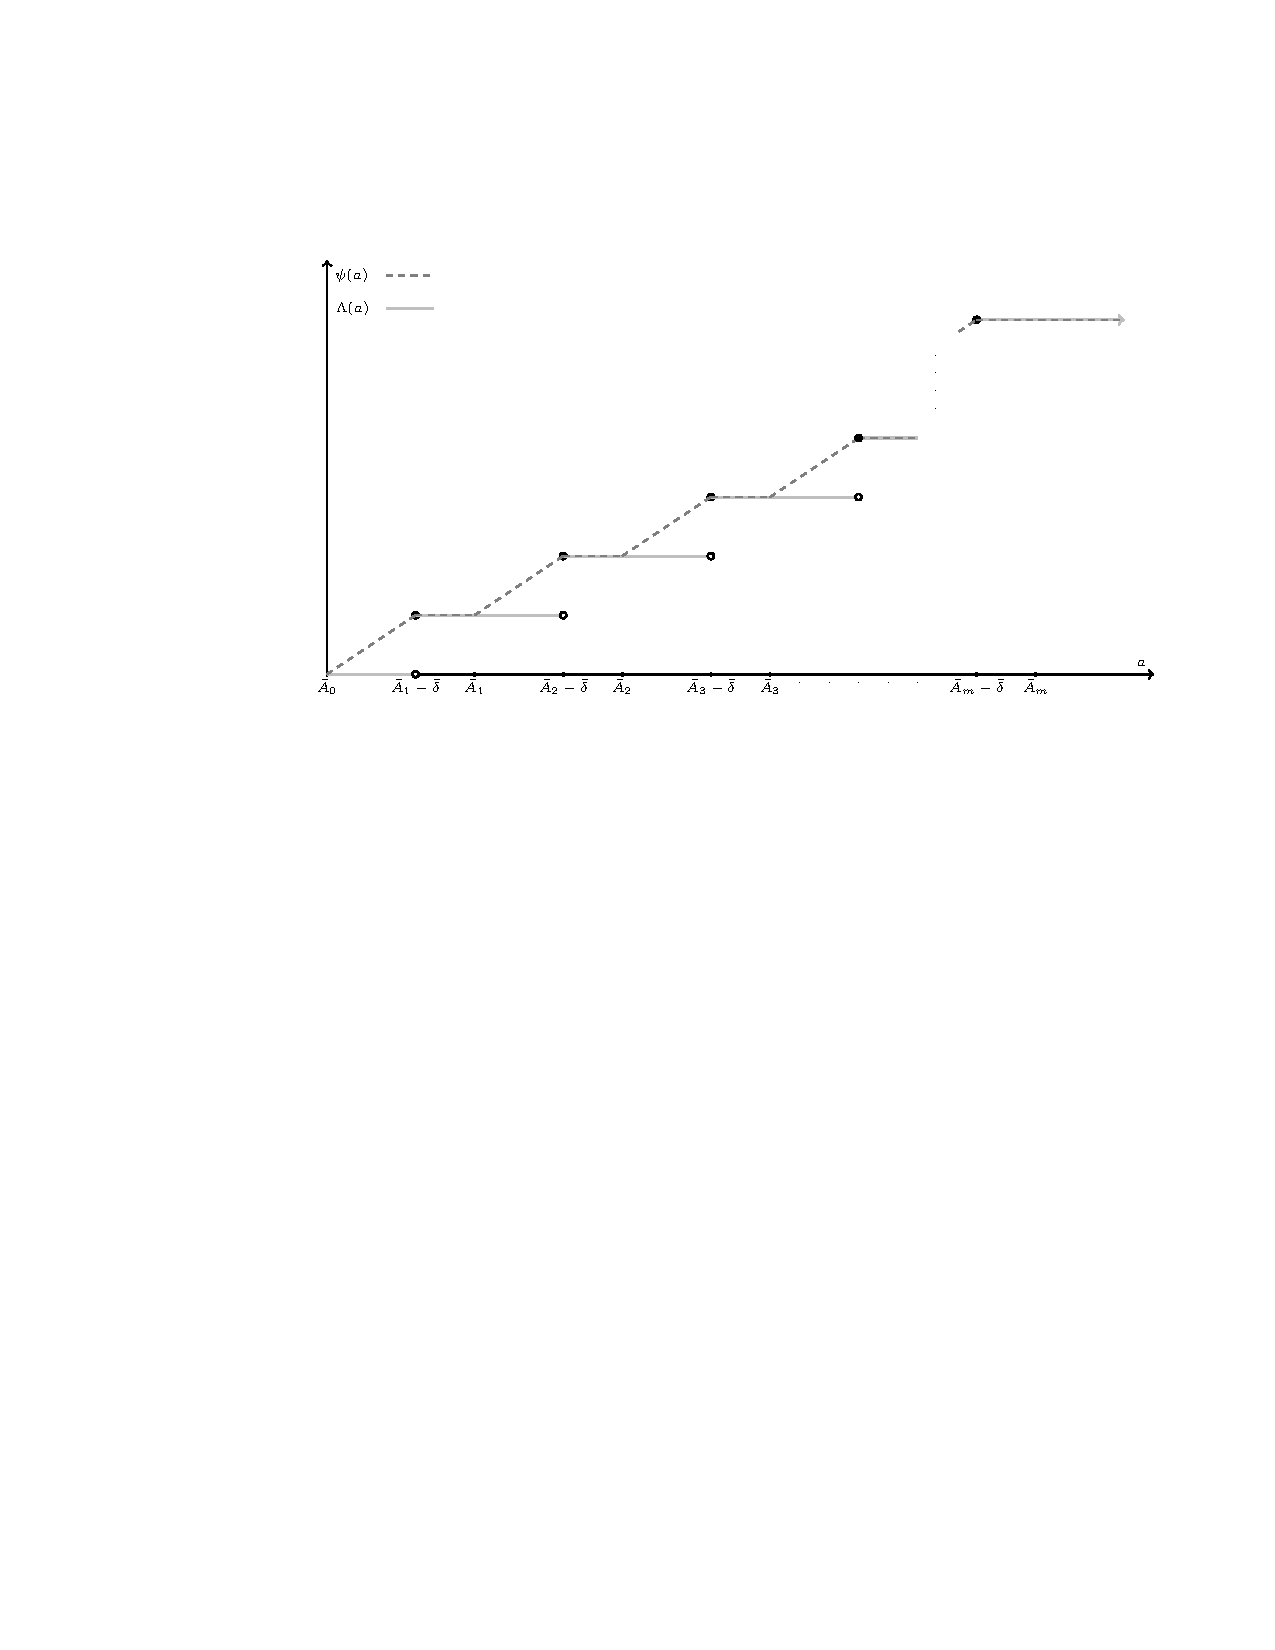
\includegraphics[scale = 1]{Subadditivebound}\\
  \caption*{\small \textsc{Figure 1}: Lifting function $\Lambda(a)$ and subadditive upper bound $\psi(a)$, $a\geq 0$}\label{fig:subadditive}
\end{figure}


\begin{prop}
  The lifted pack inequality,
    \begin{align}
        \x(N\sm \bar{P}) - \sum_{i\,\in \bar{P}} \psi(a_i) (1-x_i) \leq 0 \label{ineq:liftedpacksub}
    \end{align}
    is valid for $\conv(K)$. In addition, \eqref{ineq:liftedpacksub} defines a $n-m-1$ dimensional face of $\conv{K}$ if $A_{i_k} - \bar{\delta} \leq a_{k} \leq A_{i_k}$, for some $i_k \in \{0,1,2,\ldots, m-1\}$ for all $k \in \bar{P}$.
\end{prop}

As in the case of cover inequalities, a computationally inexpensive procedure to lift maximal pack inequalities is to identify whether a variable $x_i,\,i\in \bar{P}$ can be introduced into the maximal pack inequality with a coefficient $\alpha_i \geq 1$. Let $E$ be a set of all such indices, i.e. $E \define \set{i\inset \bar{P}}{\alpha_i \geq 1}$. The extended pack inequality thus is,
\begin{align}
    \x(E \cup (N\sm \bar{P})) \leq |E| \label{ineq:extdpack}
\end{align}

Consider a subset of indices $\bar{E} \subseteq \bar{P}$. Assume that the corresponding variables $x_i,\,i\in \bar{E}$ have been included in the extended cover inequality. Consider the variable $x_k, k \in \bar{P}\sm \bar{E})$ to be included next in the extended cover.

\begin{prop}
  $\alpha_k \geq 1,$ if $a_k + \bar{\delta} \geq \underset{j\in N\sm \bar{P}}{\max}\, a_j$.
\end{prop}
where $\bar{\delta}\define b - a(\bar{P})$ is the residual capacity of the maximal pack. The corresponding extension set $E \subseteq \bar{P}$ can now be defined as,
\begin{align}
\label{set:packext}
        E \define \set{i\inset \bar{P}}{a_i + \bar{\delta} \geq \underset{j\in N\sm \bar{P}}{\max}\, a_j}
\end{align}

\begin{prop}
  The extended pack inequality \eqref{ineq:extdpack} is valid for $\conv(K_{\bar{P}\sm E})$. In addition, inequality \eqref{ineq:extdpack} defines a facet of $\conv(K_{\bar{P}\sm E})$ if and only if $\bar{P}$ is maximal and $\forall\, i\inset E$ $\exists\, \text{distinct }\{j,k\}\inset N\sm \bar{P}$ such that $\a(\bar{P}\cup \{j,k\}\sm \{i\}) > b$.
\end{prop}

\subsubsection{Sequence Independent Bounds on the Lifting Coefficients}\hfill

As in the case of covers, it is of interest to determine sequence independent bounds on the lifting coefficients of the lifted pack inequality \eqref{ineq:liftedpack}. The particular bounds can be obtained using the lifting function $\Lambda(\cdot)$ and the subadditive upper bound $\psi(\cdot)$. Observe that any feasible solution to $\max\set{\x(N\sm \bar{P})}{\sum_{i \in N\sm \bar{P}} a_i x_i \leq \bar{\delta} + a_j}$ provides a lower bound on the lifting coefficient $\alpha_j,\, j \in \bar{P}$. Alternatively, the subadditive upper bound $\psi(a_j)$ yields an upper bound on $\alpha_j,\, j \in \bar{P}$. Consider the following,

\begin{prop}
\label{prop:seqindpacks}
  Suppose that $\bar{P} \subseteq N$ is a maximal pack, and the lifted pack inequality \eqref{ineq:liftedpack} defines a $n-m-1$ dimensional face of $\conv(K)$, then the following statements hold for all $\alpha_j,\, j \in \bar{P}$,
  \begin{enumerate}[label=(\roman{*})]
    \item $\alpha_j \leq h$, if $a_j \leq \bar{A}_h$.
    \item $\alpha_j \geq h$, if $a_j \geq \bar{B}_h - \bar{\delta}$.
  \end{enumerate}
\end{prop}
\begin{proof}
  $(i)$ Follows from the definition of subadditive upper bound $\psi(a_j),\,j \in \bar{P}$.\\
  $(ii)$ Consider $T \subseteq S$ such that $|T| = h$. Observe that, for $j \in \bar{P}$, $\alpha_j \geq h$, if $a(T) \leq \bar{\delta} + a_j$ for all possible lifting sequences. In other words,
  \begin{align*}
    \alpha_j \geq h & \hspace{4mm} \text{ if } \underset{\substack{T\subseteq N\sm \bar{P}\\|T| = h}}{\max}\,\, \a(T) \leq a_j + \bar{\delta}\\
    \alpha_j \geq h & \hspace{4mm} \text{ if } \bar{B}_h \leq a_j + \bar{\delta}.
  \end{align*}
  The result follows.
\end{proof}

\begin{cor}
  The extended pack inequality,
  \begin{align}
    \x(N\sm \bar{P}) + \sum_{j \in \bar{P}}c_j x_j \leq \mathbf{c}(\bar{P})
  \end{align}
  is valid for $\conv(K)$, where $c_j = h,$ if $\bar{A}_h \leq a_j \leq \bar{B}_h - \bar{\delta},\,\,j\in \bar{P}$ .
\end{cor}
\subsection{Generalizing the linear 0-1 knapsack}

In this section, we present a more general expression for the cover inequalities whilst relaxing the earlier assumption of $\a > 0$. While this is a trivial exercise for the reader, and these expressions can be readily obtained via complementing variables $x_i$ where corresponding $a_i < 0$, we present the following results to provide a sense of completeness to this analysis.

Reconsider the knapsack set $K$, with $\a\in \R$.

Define the indexed sets, $I^+$ and $I^-$ as following,
\begin{align*}
      I^+ \define \set{i \in N}{a_i > 0}\hspace{0.5cm} I^- = N\sm I^+ \define \set{i \in N}{a_i < 0}
\end{align*}
The knapsack set $K$ can be redefined for the aforementioned indexed sets as following,
\begin{align}
    K = \set{\x \in \binset^n}{\sum_{i\in I^+} a_ix_i + \sum_{j\in I^-} |a_j|\bar{x}_j \leq b + \sum_{j\in I^-} |a_j|}\label{set:genknapsack}
\end{align}
where $\bar{x}_j = 1-x_j,\,\forall\,j\inset I^-$.

\begin{prop}
  Inequality $x_i \geq 0$, $i\in I^+$ is facet defining for $\conv(K)$.
\end{prop}

\begin{prop}
  Inequality $x_i \leq 1$, $i\in I^-$ is facet defining for $\conv(K)$.
\end{prop}

\begin{prop}
  Inequality $x_i \leq 1$, $i\in I^+$ is facet defining for $\conv(K)$ if and only if $a_i + |a_k| \leq b + |\a|(I^-) $, $\forall\,\,k\inset N\setminus\{i\}$.
\end{prop}

\begin{prop}
  Inequality $x_i \geq 0$, $i\in I^-$ is facet defining for $\conv(K)$ if and only if $|a_i| + |a_k| \leq b + |\a|(I^-)$, $\forall\,\,k\inset N\setminus\{i\}$.
\end{prop}

\begin{prop}
  If the inequality $\boldsymbol\alpha\x \leq \beta$ defines a facet for $\conv(K)$ not including $\mathbf{0}$ then $\beta > \boldsymbol\alpha(I^-)$, $\alpha_i \geq 0$, $\forall\,\,i\in I^+$ and $\alpha_j \leq 0$, $\forall\,\,j\in I^-$.
\end{prop}

\subsubsection{Cover Inequalities, $\a \in \R$}\label{sec:gencover}\hfill

Consider sets, $C^+ \subseteq I^+$ and $C^- \subseteq I^-$, such that $C^+ \cup C^-$ constitutes a cover, i.e.
\begin{align*}
  \hspace*{4cm}\sum_{i\in C^+} a_i &+ \sum_{j\in C^-} |a_j| & & > b + \sum_{j\in I^-} |a_j| &\hspace*{5cm}\\
  \hspace*{4cm}\sum_{i\in C^+} a_i &- \sum_{j\in I^-\sm C^-} |a_j| & & > b &\hspace*{5cm}\\
  \hspace*{4cm}\sum_{i\in C^+} a_i &+ \sum_{j\in I^-\sm C^-} a_j & & > b &\hspace*{5cm}\\
  \hspace*{4cm}&\sum_{i\in C^+\cup I^-\sm C^-} a_i & & > b. &\hspace*{5cm}\\
\end{align*}
then, the corresponding cover inequality can be expressed as,
\begin{align*}
    \sum_{i\in C^+} x_i + \sum_{j\in C^-} \bar{x}_j & \leq |C^+ \cup C^-| - 1\\
    \sum_{i\in C^+} x_i + \sum_{j\in C^-} (1 - {x}_j) & \leq |C^+| + |C^-| - 1\\
    \sum_{i\in C^+} x_i - \sum_{j\in C^-} x_j + |C^-| & \leq |C^+| + |C^-| - 1\\
    \sum_{i\in C^+} x_i - \sum_{j\in C^-} x_j  & \leq |C^+| - 1
\end{align*}
The following result follows,
\begin{prop}
  The \emph{generalized cover inequality},
    \begin{align}
    \label{ineq:gencover}
      \x(C^+) - \x(C^-) \leq |C^+| - 1
    \end{align}
  is valid for $\conv(K)$. Furthermore, inequality \eqref{ineq:gencover} defines a facet for $\conv{K_{C^+ \cup C^-}}$ if and only if $C^+\cup C^-$ is of minimal cardinality, i.e.
  \begin{align*}
    |a_i| \geq \lambda,\,\,\,\, \forall\,\, i \in C^+\cup C^-
  \end{align*}
\end{prop}
It can also be seen that the corresponding the generalized lifted cover inequality in this case can be represented as,
\begin{align*}
        &\x(C^+) + \sum_{i\,\in I^+\sm C^+} \alpha_i x_i + \sum_{j\,\in I^-\sm C^-} \alpha_j \bar{x}_j- \x(C^-) \leq |C^+| - 1\\
        &\x(C^+) + \sum_{i\,\in I^+\sm C^+} \alpha_i x_i + \sum_{j\,\in I^-\sm C^-} \alpha_j (1-{x}_j) - \x(C^-) \leq |C^+| - 1\\
        &\x(C^+) + \sum_{i\,\in I^+\sm C^+} \alpha_i x_i - \sum_{j\,\in I^-\sm C^-} \alpha_j x_j - \x(C^-) \leq |C^+| - \boldsymbol\alpha(I^-\sm C^-) - 1
\end{align*}
which yields the generalized lifted cover inequality,
\begin{align}
\label{ineq:genliftedcover}
    \x(C^+) + \sum_{i\,\in I^+\sm C^+} \alpha_i x_i - \sum_{j\,\in I^-\sm C^-} \alpha_j x_j - \x(C^-) \leq |C^+| - (\boldsymbol\alpha(I^-\sm C^-) + 1)
\end{align}
where $\alpha_i \geq 0,\,i\in I^+\sm C^+$ and $\alpha_j \geq 0,\,j\in I^-\sm C^-$ are the corresponding lifting coefficients. Let $E$ be a set of all such indices, i.e. $E \define \set{i\inset N\sm (C^+ \cup C^-)}{\alpha_i \geq 1}$.

%Consider a permutation of the indices in the complement set $N\sm (C^+ \cup C^-)$. Let $\{(1),(2),\ldots,(|N\sm (C^+ \cup C^-)|)\}$ be the permutation of elements of the set $N\sm (C^+ \cup C^-)$. Define $C_k \define (C^+ \cup C^-) \cup \{(1),(2),\ldots,(k)\},\, 0\leq k\leq |N\sm (C^+ \cup C^-)|$ with $C_0 = (C^+ \cup C^-)$. The extension $E$ with respect to $(C^+ \cup C^-)$ can be represented as,
%\begin{align}
%  E \define \set{(k) \in N\sm (C^+ \cup C^-)}{|a_{(k)}| > \underset{j\in C_{k-1}}{\max}\, |a_j| - \lambda_{k-1}}
%\end{align}
%where $\lambda_k = \lambda_{k-1} - \left(\underset{j\in C_{k-1}}{\max}\, |a_j| - |a_{(k)}|\right)^+$ and $\lambda_0 = b - \underset{i\in C^+\cup (I^-\sm C^-)}{\sum}\, a_i$

Sequence independent extensions for this generalization can also be obtained in a manner similar to Section \ref{sec:extension}. We characterize the extension set $E$ with respect to $(C^+ \cup C^-)$ as,
\begin{align}
\label{set:extplus}
    E \define \set{i\inset N\sm (C^+\cup C^-)}{|a_i| > \underset{j\in C^+\cup C^-}{\max}\, |a_j| - \lambda}
\end{align}
where $\lambda = \a(C^+\cup (I^-\sm C^-)) - b$.

Further define subsets $E^+$ and $E^-$ as,
\begin{align*}
  E^+ \define I^+ \cap E \hspace{5mm} E^- \define I^- \cap E
\end{align*}

The \emph{generalized extended cover inequality} can now be expressed as,
\begin{align*}
        \x(C^+\cup E^+) + \bar{\x}(C^-\cup E^-) & \leq |C^+| + |C^-| - 1\\
        \x(C^+\cup E^+) + |C^-\cup E^-| - \x(C^-\cup E^-) & \leq |C^+| + |C^-| - 1\\
        \x(C^+\cup E^+) + |C^-| + |E^-| - \x(C^-\cup E^-) & \leq |C^+| + |C^-| - 1\\
        \x(C^+\cup E^+) - \x(C^-\cup E^-) & \leq |C^+| - (|E^-| + 1)
\end{align*}

The result follows,

\begin{prop}
\label{prop:genextcover}
  The generalized extended cover inequality,
  \begin{align}
    \label{ineq:genextcover}
    \x(C^+\cup E^+) - \x(C^-\cup E^-) \leq |C^+| - (|E^-| + 1)
  \end{align}
  is valid for $\conv(K)$. In addition, inequality \eqref{ineq:genextcover} defines a facet of $\conv(K_{C^+\cup C^-\cup E^+ \cup E^-})$ if and only if $C^+\cup C^-$ is of minimal cardinality and $\forall\, i\inset E^+\cup E^-$ $\exists\, \text{distinct }\{j,k\}\inset C^+\cup C^-$ such that $|\a|(C^+\cup C^- \cup \{i\} \sm \{j,k\}) \leq b + |\a|(I^-)$
\end{prop}

\subsubsection{Sequence Independent Bounds on Lifting Coefficients}\hfill

%-------------------------------------------
%As a direct generalization of the results presented in Section \ref{sec:seqindp} we present the following conditions to provide sequence independent bounds on the lifting coefficients of the lifted cover inequality \eqref{ineq:genliftedcover},
%\begin{align*}
%    \x(C^+) + \sum_{i\,\in I^+\sm C^+} \alpha_i x_i - \sum_{j\,\in I^-\sm C^-} \alpha_j x_j - \x(C^-) \leq |C^+| - (\boldsymbol\alpha(I^-\sm C^-) + 1)
%\end{align*}
%where $\alpha_i \geq 0,\,i\in I^+\sm C^+$ and $\alpha_j \geq 0,\,j\in I^-\sm C^-$ are the corresponding lifting coefficients.
%
%To obtain the lower bounds on the aforementioned lifted coefficients, we use the alternate representation of the linear $0-1$ knapsack \eqref{set:genknapsack}, then Proposition \ref{prop:seqindlowbound} readily yields the following result.
%\begin{prop}
%  Let $(C^+ \cup C^-) \subset N$ be a cover with $\lambda \define b - \underset{i\in C^+\cup (I^-\sm C^-)}{\sum}\, a_i$. Suppose that the lifted pack inequality \eqref{ineq:genliftedcover} defines a facet of $\conv(K)$. Then, for $k\in N\sm (C^+ \cup C^-),$ $\alpha_k \geq h,$ if $|a_k| \geq A_h$, where $A_h = \underset{\substack{T\subseteq C^+ \cup C^-\\|T| = h}}{\max}\,\, |\a|(T)$
%\end{prop}
%
%Similarly, Proposition \ref{prop:seqindupbound} can be extended to this case to yield upper bounds on the lifting coefficients, $\alpha_i,\, i \in N\sm (C^+ \cup C^-)$
%\begin{prop}
%  Let $(C^+ \cup C^-) \subset N$ be a cover with $\lambda \define b - \underset{i\in C^+\cup (I^-\sm C^-)}{\sum}\, a_i$. Suppose that the lifted pack inequality \eqref{ineq:genliftedcover} defines a facet of $\conv(K)$. Then, for $k\in N\sm (C^+ \cup C^-),$ $\alpha_k \leq h,$ if $|a_k| \leq b + |\a|(I^-) - B_{|C^+ \cup C^-|-1-h}$, where $B_h = \underset{\substack{T\subseteq C^+ \cup C^-\\|T| = h}}{\min}\,\, |\a|(T)$.
%\end{prop}
%------------------------------------
As a direct generalization of the results presented in Section \ref{sec:seqindp} we present the following conditions to provide sequence independent bounds on the lifting coefficients of the lifted cover inequality \eqref{ineq:genliftedcover},
\begin{align*}
    \x(C^+) + \sum_{i\,\in I^+\sm C^+} \alpha_i x_i - \sum_{j\,\in I^-\sm C^-} \alpha_j x_j - \x(C^-) \leq |C^+| - (\boldsymbol\alpha(I^-\sm C^-) + 1)
\end{align*}
where $\alpha_i \geq 0,\,i\in I^+\sm C^+$ and $\alpha_j \geq 0,\,j\in I^-\sm C^-$ are the corresponding lifting coefficients.

To obtain the lower bounds on the aforementioned lifted coefficients, we use the alternate representation of the linear $0-1$ knapsack \eqref{set:genknapsack}. Proposition \ref{prop:seqindlowbound} and Proposition \ref{prop:seqindupbound} can be readily extended to this case to yield lower and upper bounds on the lifting coefficients, $\alpha_i,\, i \in N\sm (C^+ \cup C^-)$.

\begin{dfn}
  Let $(C^+ \cup C^-)\subset N$ be of minimal cardinality such that $$\a(C^+ \cup (I^-\sm C^-)) > b.$$ For $h = 0,1,2,3,\ldots,|(C^+ \cup C^-)|$, define,
  \begin{align}
    A_h \define \max \,\set{|\a|(T)}{T \inset \mathcal{T}_h} \label{def:Ah}\\
    B_h \define \min \,\set{|\a|(T)}{T \inset \mathcal{T}_h} \label{def:Bh}
  \end{align}
  where $\mathcal{T}_h \define \set{T}{|T| = h,\,\, T \subseteq (C^+ \cup C^-)}$.
\end{dfn}

\begin{prop}
  Let $(C^+ \cup C^-) \subset N$ be a cover with $\lambda \define \a(C^+\cup (I^-\sm C^-)) - b$ and $A_h$ and $B_h$, $h = 0,1,2,3,\ldots,|C^+ \cup C^-|$ be defined as in \eqref{def:Ah} and \eqref{def:Bh}. Suppose that the lifted pack inequality \eqref{ineq:genliftedcover} defines a facet of $\conv(K)$. Then, for $k\in N\sm (C^+ \cup C^-),$ the following statements hold,
  \begin{enumerate}[label=(\roman{*})]
    \item If $|a_k| \geq A_h$, then $\alpha_k \geq h$.
    \item If $|a_k| \leq b + |\a|(I^-) - B_{|C^+ \cup C^-|-1-h}$, then $\alpha_k \leq h$
  \end{enumerate}
\end{prop}

\subsubsection{Pack Inequalities, $\a \in \R$}\hfill

\label{sec:genpack}
Akin to the cover inequalities presented for $K,\,\a\in \R$ above, we can rewrite the pack inequalities similarly, i.e. \textit{(via. complementation)}

Reconsider the knapsack set $K$, with $\a\in \R$. Apropos of the index sets $I^+$ and $I^-$ and corresponding feasible set $K$ \eqref{set:genknapsack} defined earlier in Section \ref{sec:gencover}

Consider now, $P^+ \subseteq I^+$ and $P^- \subseteq I^-$, such that $P^+ \cup P^-$ defines a pack, i.e.,
\begin{align*}
  \hspace*{4cm}\sum_{i\in P^+} a_i &+ \sum_{j\in P^-} |a_j| & & < b + \sum_{j\in I^-} |a_j| &\hspace*{5cm}\\
  \hspace*{4cm}\sum_{i\in P^+} a_i &- \sum_{j\in I^-\sm P^-} |a_j| & & < b &\hspace*{5cm}\\
  \hspace*{4cm}\sum_{i\in P^+} a_i &+ \sum_{j\in I^-\sm P^-} a_j & & < b &\hspace*{5cm}\\
  \hspace*{4cm}&\sum_{i\in P^+\cup I^-\sm P^-} a_i & & < b. &\hspace*{5cm}\\
\end{align*}
For $\delta \define b - \a(P^+\cup (I^-\sm P^-))$  and  $M \define \set{i\in N\sm (P^+\cup P^-)}{|a_i| > \delta}$, the corresponding pack inequality can be expressed as,
\begin{align*}
    \sum_{i\in M\cap I^+} x_i + \sum_{j\in M\cap I^-} \bar{x}_j & \leq 0\\
    \sum_{i\in M\cap I^+} x_i + \sum_{j\in M\cap I^-} (1 - {x}_j) & \leq 0\\
    \sum_{i\in M\cap I^+} x_i + |M\cap I^-| & \leq \sum_{j\in M\cap I^-} x_j\\
    \sum_{i\in M\cap I^-} x_i - \sum_{j\in M\cap I^+} x_j  & \geq |M\cap I^-|
\end{align*}

The following result follows,
\begin{prop}
  The \emph{generalized pack inequality},
    \begin{align}
    \label{ineq:genpack}
      \x(M\cap I^-) - \x(M\cap I^+) \geq |M\cap I^-|
    \end{align}
  is valid for $\conv(K_{P^+ \cup P^-})$. Furthermore, inequality \eqref{ineq:genpack} defines a facet for $\conv(K_{P^+ \cup P^-})$ if and only if $P^+\cup P^-$ is of maximal cardinality, i.e.
  \begin{align*}
    |a_i| > \delta,\,\,\,\, \forall\,\, i \in N\sm (P^+\cup P^-)
  \end{align*}
  or $M = N\sm (P^+\cup P^-)$
\end{prop}

In addition, attributing to the above preliminaries we can rewrite the weight inequalities for the generalized $0-1$ knapsack,
\begin{prop}
\label{prop:genweight}
  The \textit{generalized weight inequality},
  \begin{align}
    \sum_{i\in P^-} a_i x_i - \sum_{i\in P^+} a_i(1-x_i) + \sum_{j \in M\cap I^+} (a_j - \delta)^+ x_j + \sum_{j \in M\cap I^-} (-a_j - \delta)^+ (1-x_j) \leq 0
  \end{align}
  is valid for $\conv(K)$.
\end{prop}
For $\bar{P} = \bar{P}^+ \cup \bar{P}^-$ maximal and corresponding residue $\bar{\delta} = b - \a(\bar{P}^+\cup (I^-\sm \bar{P}^-))$, we have the maximal pack inequality,
\begin{align}
  \x(I^-\sm \bar{P}) - \x(I^+\sm \bar{P}) \geq |I^-\sm \bar{P}|
\end{align}
and the maximal weight inequality,
\begin{align}
  \sum_{i\in P^-} a_i x_i - \sum_{i\in P^+} a_i(1-x_i) + \sum_{j \in I^+\sm P^+} (a_j - \bar{\delta})^+ x_j + \sum_{j \in I^-\sm P^-} (-a_j - \bar{\delta})^+ (1-x_j) \leq 0
\end{align}

It can also be seen that the corresponding generalized lifted pack inequality for $\bar{P}$ maximal, can be represented as,
\begin{align*}
        &\x(I^-\sm \bar{P}) - \sum_{i\,\in \bar{P}^+} \alpha_i (1-x_i) - \x(I^+\sm \bar{P}) - \sum_{j\,\in \bar{P}^-} \alpha_j (1-\bar{x}_j) \geq |I^-\sm \bar{P}|\\
        &\x(I^-\sm \bar{P}) + \sum_{i\,\in \bar{P}^+} \alpha_i x_i - \boldsymbol\alpha(\bar{P}^+) - \x(I^+\sm \bar{P}) - \sum_{j\,\in \bar{P}^-} \alpha_j {x}_j \geq |I^-\sm \bar{P}|\\
        &\x(I^-\sm \bar{P}) + \sum_{i\,\in \bar{P}^+} \alpha_i x_i - \x(I^+\sm \bar{P}) - \sum_{j\,\in \bar{P}^-} \alpha_j {x}_j \geq |I^-\sm \bar{P}| + \boldsymbol\alpha(\bar{P}^+)\\
\end{align*}
which yields the generalized lifted pack inequality,
\begin{align}
\label{ineq:genliftedpack}
    \x(I^-\sm \bar{P}) + \sum_{i\,\in \bar{P}^+} \alpha_i x_i - \x(I^+\sm \bar{P}) - \sum_{j\,\in \bar{P}^-} \alpha_j {x}_j \geq |I^-\sm \bar{P}| + \boldsymbol\alpha(\bar{P}^+)
\end{align}
where $\alpha_i,\,i\in \bar{P}^+ \define \bar{P}\cap I^+$ and $\alpha_j,\,j\in \bar{P}^- \define \bar{P}\cap I^-$ are the corresponding lifting coefficients. Let $E$ be a set of all such indices, i.e. $E \define \set{i\inset \bar{P}}{\alpha_i \geq 1}$.

We characterize the extension set $E$ with respect to $(\bar{P}^+ \cup \bar{P}^-)$ as,
\begin{align}
\label{set:extplus}
    E \define \set{i\inset \bar{P}}{|a_i| + \bar{\delta} \geq \underset{j\in N\sm \bar{P}}{\max}\, |a_j|}
\end{align}
where $\bar{\delta} = b - \a(\bar{P}^+\cup (I^-\sm \bar{P}^-))$.

Further define subsets $E^+$ and $E^-$ as,
\begin{align*}
  E^+ \define I^+ \cap E \hspace{5mm} E^- \define I^- \cap E
\end{align*}

The \emph{generalized pack inequality} can now be expressed as,
\begin{align*}
        \x(E^+ \cup I^-\sm \bar{P}) - \x(E^- \cup I^+\sm \bar{P}) \geq |I^-\sm \bar{P}| + |E^+|
\end{align*}

The result follows,

\begin{prop}
\label{prop:genextpack}
  The generalized extended pack inequality,
  \begin{align}
    \label{ineq:genextpack}
    \x(E^+ \cup I^-\sm \bar{P}) - \x(E^- \cup I^+\sm \bar{P}) \geq |I^-\sm \bar{P}| + |E^+|
  \end{align}
  is valid for $\conv(K_{\bar{P}^+\cup \bar{P}^-\sm (E^+ \cup E^-)})$. In addition, inequality \eqref{ineq:genextpack} defines a facet of $\conv(K_{\bar{P}^+\cup \bar{P}^-\sm (E^+ \cup E^-)})$ if and only if $\bar{P}$ is of maximal cardinality and $\forall\, i\inset E$ $\exists\, \text{distinct }\{j,k\}\inset N\sm \bar{P}$ such that $|\a|(\bar{P}\cup \{j,k\}\sm \{i\}) > b  + |\a|(I^-)$
\end{prop}

%\subsubsection{Sequence Independent Bounds on Lifting Coefficients}\hfill
The extended pack inequalities are often valid for low dimensional extensions of the knapsack set and not the original set itself. Lifting the pack inequalities yields us strong inequalities that are valid for the convex hull of the original knapsack set, $\conv(K)$. The lifted pack inequality for the generalized linear $0-1$ knapsack can be expressed as \eqref{ineq:genliftedpack},
\begin{align*}
  \x(I^-\sm \bar{P}) + \sum_{i\,\in \bar{P}^+} \alpha_i x_i - \x(I^+\sm \bar{P}) - \sum_{j\,\in \bar{P}^-} \alpha_j {x}_j \geq |I^-\sm \bar{P}| + \boldsymbol\alpha(\bar{P}^+)
\end{align*}
where $\bar{P}$ represents a maximal pack, and $\alpha_i \geq 0,\,i\in \bar{P}^+$ and $\alpha_j \geq 0,\,j\in \bar{P}^-$ are the corresponding lifting coefficients.

Sequence independent bounds on the aforementioned lifting coefficients can be obtained as a direct generalizations of Proposition \ref{prop:seqindpacks}, the results follows,
\begin{prop}
  Suppose that $\bar{P} \subseteq N$ is a maximal pack. Let $m = |N\sm \bar{P}|$ and suppose the lifted pack inequality \eqref{ineq:liftedpack} defines a $n-m-1$ dimensional face of $\conv(K)$, then the following statements hold for all $\alpha_j,\, j \in \bar{P}$,
  \begin{enumerate}[label=(\roman{*})]
    \item $\alpha_j \leq h$, if $|a_j| \leq \bar{A}_h$.
    \item $\alpha_j \geq h$, if $|a_j| \geq \bar{B}_h - \bar{\delta}$.
  \end{enumerate}
  where $\bar{A}_h = \min\set{\a(T)}{T\subseteq N\sm \bar{P},\,|T| = h}$ and $\bar{B}_h = \max\set{\a(T)}{T\subseteq N\sm \bar{P},\,|T| = h}$ for $h = 0, 1,2,\ldots, m$ and the excess $\bar{\delta} = b - \a(\bar{P}^+ \cup (I^+\sm \bar{P}^-)) $
\end{prop}

\begin{cor}
  The extended generalized pack inequality,
  \begin{align}
    \x(I^-\sm \bar{P}) + \sum_{i\,\in \bar{P}^+} c_i x_i - \x(I^+\sm \bar{P}) - \sum_{j\,\in \bar{P}^-} c_j {x}_j \geq |I^-\sm \bar{P}| + \mathbf{c}(\bar{P}^+)
  \end{align}
  is valid for $\conv(K)$, where $c_j = h,$ if $\bar{A}_h \leq a_j \leq \bar{B}_h - \bar{\delta},\,\,j\in \bar{P}$ .
\end{cor}

\section{Generalizations to Submodular Knapsacks}
In this section we will extend the results of the $0-1$ linear knapsack to submodular knapsacks. Consider a set function $f : \binset^n \mapsto \R$, $f(\emptyset) = 0$. For $f$ submodular on a finite set $N$ and $b \in \R$, we define the submodular knapsack set $K^f$ as lower level set of $f$,
$$
    K^f = \set{\x \in \binset^n}{f(\x) \leq b}
$$
A special case for the submodular knapsack polytope, namely when $f$ is non-decreasing on $N$ has been studied by \atam and Narayanan \cite{Atamturk2009333} where they derive cover inequalities and their extensions for this special case. The generalization of cover inequalities to this special case, although interesting appears to lack the understanding of their \textit{evolution}. It also appears that the general submodular knapsack has not been studied yet in the literature. In this particular section we will present the corresponding valid inequalities and their extensions for the generalized submodular polytope $\conv(K^f)$, whilst also providing an understanding \emph{vis-\`{a}-vis} how these inequalities can be derived from the conjunction of two of the main understandings for knapsacks and submodular functions, namely the cover inequalities and the extended polymatroids. These inequalities per our understanding serve as the most generalized version of the cover and pack inequalities for the knapsack polytope.

\subsection{Submodular functions and Extended Polymatroids}
\begin{dfn}
  Let $f:\binset^n \mapsto \R$ be a submodular set function on a finite set $N$. The set $EP_f$ is called the extended polymatroid associated with $f$, where,
  $$
        EP_f \define \set{\bv\in \R^n}{\bv(S) \leq f(S),\,\,S\subset N}.
  $$
\end{dfn}

\begin{thm}
   (Edmonds, 1970) \cite{edmonds03} For any submodular function $f$ on a finite set $N$ $(f(\emptyset) = 0)$, the vertices of the extended polymatroid $EP_f$ are given by,
   $$
        v^{\bpi}_j = f(S^{\bpi}_j) - f(S^{\bpi}_{j-1}),
   $$
   for a permutation $\bpi$ of $\{1,2,\ldots, n\}$, and $S^{\bpi}_j$ denotes the set consisting of first $j$ elements of the permutation $\bpi$.
\end{thm}

\begin{dfn}
  Let $\mathbf{V}_f$ denote the set of all extreme points of $EP_f$.
\end{dfn}

\begin{cor}
\label{cor:extpolymat}
    Consider the following set,
    $$
        B \define \set{(\x, z) \in \binset^n\times \R}{f(x)\leq z}
    $$
    then $$\bv \x \leq z, \,\,\bv \in EP_f$$ is valid for $B$. In particular, $\bv \x \leq z$ defines a facet of $B$ for all $\bv \in \mathbf{V}_f$.
\end{cor}

%\begin{cor}
%  Define the two level sets $K_1$ and $K_2$ as following for some $\gamma \in \R$,
%  \begin{align*}
%      K_1 = \set{x\in \binset^n}{f(\x) \leq \gamma}\hspace{0.5cm} K_2 = \set{x\in \binset^n}{\bv\x \leq \gamma, \,\,\bv \in \mathbf{V}_f}
%  \end{align*}
%  then $K_1 = K_2$.
%\end{cor}

\begin{cor}
  Define, for some $\gamma \in \R$, $K_{\bv} \define \set{\x \in \binset^n}{\bv \x \leq \gamma}$ for some $\bv \in \mathbf{V}_f$ and $K_{f} \define \set{\x \in \binset^n}{f(\x) \leq \gamma}$.
  \begin{enumerate}[label=\emph(\roman{*})]
    \item $\underset{\bv\inset \mathbf{V}_f}{\bigcap}\, K_{\bv} = K_f$
    \item If $\boldsymbol\alpha \x \leq \beta,\,$ is valid for $K_{\bv}$ for some $\bv \in \mathbf{V}_f$ then $\boldsymbol\alpha \x \leq \beta$ is valid for $K_{f}$.
    \item If $\boldsymbol\alpha \x \leq \beta$ defines a facet of $K_{\bv}$ for some $\bv \in \mathbf{V}_f$ and $\exists$ $\x^1, \x^2, \ldots, \x^k,$ $1\leq k \leq n$ affinely independent points on the hyperplane $\boldsymbol\alpha \x = \beta$ satisfying $f(\x^i) \leq b,\,1\leq i \leq k$ then $\boldsymbol\alpha \x \leq \beta$ defines a $k-1$ dimensional face of $K_f$. In particular, when $k=n$, $\boldsymbol\alpha \x \leq \beta$ defines a facet of $K_f$.
    \item Let $\boldsymbol\alpha\x \leq \beta_{\bv}$ imply that the set of conditions $\Gamma$ are satisfied for some $K_{\bv},\,\, \bv \inset \mathbf{V}_f$. If $\exists\,\, \beta < \beta_{\bv}\,\,\forall\,\,\bv \inset \mathbf{V}_f$, then $\Gamma$ are satisfied for $K_{f}$ if $\boldsymbol\alpha\x \leq \beta$.
  \end{enumerate}
\end{cor}

\subsection{Valid Inequalities for $K^f$}\hfill

As earlier, let $f : \binset^n \mapsto \R$ be a submodular set function on a finite set $N$. Also let $\mathbf{V}_f$ denote the set of all extreme points of the extended polymatroid of $f$, $EP_f$. Moreover, for $N$, define a permutation $\bpi$ for the elements of $N$,
$$
    \bpi \define \{(1), (2), (3),\ldots, |N|\}
$$
Also, define $S\subseteq N$ as,
\begin{align}
    S \define \{(1), (2), \ldots, (|S|)\}
\end{align}
Observe that $\sum_{(i) \in S} v^{\bpi}_i = f(S)$. For the permutation $\bpi$, define the index sets $I_{\bpi}$ and $J_{\bpi}$ as following,
\begin{align*}
  I_{\bpi} = \set{(i)\in \bpi}{v^{\bpi}_{(i)} > 0}\\
  J_{\bpi} = \set{(j) \in \bpi}{v^{\bpi}_{(i)} < 0}
\end{align*}

In addition define the sets, $I^+$ and $I^-$ as,
\begin{align*}
  I^{+} &= \set{i\in N}{\rho_i(N\sm i) > 0}\\
  I^{-} &= \set{j\in N}{\rho_i(\emptyset) < 0}
\end{align*}

One can easily observe that $I^{+} \subseteq I_{\bpi}$ and $I^{-} \subseteq J_{\bpi}$. We begin our subsequent discussion on valid inequalities for $K_f$ by presenting the results on the trivial facets of the $K^f$,

\begin{prop}
  Inequality $x_i \geq 0$, $i\in I^+$ is facet defining for $\conv(K^f)$.
\end{prop}

\begin{prop}
  Inequality $x_i \leq 1$, $i\in I^-$ is facet defining for $\conv(K^f)$.
\end{prop}

\begin{prop}
  Inequality $x_i \leq 1$, $i\in I^+$ is facet defining for $\conv(K^f)$ if and only if $f(i) + |\rho_{j}(i)| \leq b + |f(I^-)| $, $\forall\,\,k\inset N\setminus\{i\}$.
\end{prop}

\begin{prop}
  Inequality $x_i \geq 0$, $i\in I^-$ is facet defining for $\conv(X)$ if and only if $|f(i)| + |\rho_{j}(i)| \leq b + |f(I^-)| $, $\forall\,\,k\inset N\setminus\{i\}$.
\end{prop}

% Notice that |f(I^-)| = -f(I^-),

\begin{prop}
  If the inequality $\boldsymbol\alpha\x \leq \beta$ defines a facet for $\conv(X)$ not including $\mathbf{0}$ then $\beta > \boldsymbol\alpha(I^-)$, $\alpha_i \geq 0$, $\forall\,\,i\in I^+$ and and $\alpha_j \leq 0$, $\forall\,\,j\in I^-$.
\end{prop}

\subsubsection{Cover Inequalities}
\label{sec:submodcover}
\hfill

Corollary \ref{cor:extpolymat} suggests that for $\mathbf{v} \in \mathbf{V}$ of elements of $N$, $\bv \x \leq b$ is valid for $K^f$. Analogous to our discussion of the general $0-1$ linear knapsack, define the sets $C^+_{\bpi} \subseteq I_{\bpi}$ and $C^-_{\bpi} \subseteq J_{\bpi}$,
\begin{align*}
  C^+_{\bpi} \define I_{\bpi} \cap S\\
  C^-_{\bpi} \define J_{\bpi} \cap S
\end{align*}
\begin{dfn}
  We define $S\subseteq N$, $S \define \{(1), (2), \ldots, (|S|)\}$ for some permutation $\bpi = \{(1), (2), (3),\ldots, |N|\}$ as a \emph{submodular cover} if $f(S) > b$. The corresponding excess is $\lambda \define f(S) - b > 0$.
\end{dfn}
\begin{prop}
  Consider $S\subseteq N$, $S \define \{(1), (2), \ldots, (|S|)\}$ for some permutation of $\bpi = \{(1), (2), (3),\ldots, |N|\}$, then $S$ is a submodular cover if and only if $S$ is an extended polymatroid cover.
\end{prop}
\begin{proof}
  The proof follows from the definitions.
  Let $S$ be an extended polymatroid cover, thus,
  \begin{align*}
    b & < \bv(S) = \sum_{i\in S} v^{\bpi}_{i}\\
      & = \sum_{(i)\in S} f(\{S^{\bpi}_i\}) - f(\{S^{\bpi}_{i-1}\})\\
      & = f(S) - f(\emptyset)\\
      & = f(S)
  \end{align*}
  Conversely, let $S$ be a submodular cover, i.e.
  \begin{align*}
    b & < f(S) = f(S) - f(\emptyset)\\
      & = f(S^{\bpi}_{|S|}) - \sum_{j = 1}^{|S|-1}(f(S^{\bpi}_{j}) - f(S^{\bpi}_{j})) - f(\emptyset)\\
      & = \sum_{j = 1}^{|S|}(f(S^{\bpi}_{j}) - f(S^{\bpi}_{j-1}))\\
      & = \sum_{j = 1}^{|S|} v^{\bpi}_j = \bv(S)
  \end{align*}
  The result follows.
\end{proof}

\begin{dfn}
  We define $S\subseteq N$, $S \define \{(1), (2), \ldots, (|S|)\}$ for some permutation $\bpi = \{(1), (2), (3),\ldots, |N|\}$ as a \emph{minimal submodular cover} if, {\revise{minimal submodular cover with respect to $\bpi$ if,}}
  \begin{align*}
    & f(S\cup (j)) \leq b,\,\,\forall\,(j) \inset J_{\bpi}\sm C^-_{\bpi} \text{   and },\\
    & f(S\,\sm\, (i)) \leq b,\,\,\forall\,(i) \inset C^+_{\bpi}
  \end{align*}
\end{dfn}

\begin{prop}
  Consider $S\subseteq N$, $S \define \{(1), (2), \ldots, (|S|)\}$ for some permutation of $\bpi = \{(1), (2), (3),\ldots, |N|\}$, then $S$ is a minimal extended polymatroid cover if $S$ is a minimal submodular cover {\revise{with respect to $\bpi$}}.
\end{prop}
\begin{proof}
  Notice that, for $S$ to be a minimal extended polymatroid cover,
  \begin{align*}
    & \sum_{i\in S} v_i + v_j \leq b,\,\,\forall\,\,j\in C^-_{\bpi}  \text{   and },\\
    & \sum_{i\in S} v_i - v_j \leq b,\,\,\forall\,\,j\in C^+_{\bpi}
  \end{align*}
  In other words,
  \begin{align*}
     -v_j & \geq \lambda,\,\,\forall\,\,j\in C^-_{\bpi}  \text{   and },\\
     v_j & \geq \lambda,\,\,\forall\,\,j\in C^+_{\bpi}
  \end{align*}

  If $S$ is a minimal submodular cover then,
  \begin{align*}
    -\rho_{(j)}(S)  \geq \lambda,\,\,\forall\,(j) \inset J_{\bpi}\sm C^-_{\bpi}\,\,\text{ and } & \rho_{(j)}(S\sm (j)) \geq \lambda,\,\,\forall\,(j) \inset C^+_{\bpi}
  \end{align*}
  Since, $f$ is submodular, the difference function $\rho(\cdot)$ is a non-increasing function, which yields,
  $$
        v^{\bpi}_{(j)} \leq  \rho_{(j)}(S),\,\,\forall\,(j) \inset J_{\bpi}\sm C^-_{\bpi}\,\,\text{ and }  v^{\bpi}_{(j)} \geq \rho_{(j)}(S\sm (j)),\,\,\forall\,(j) \inset C^+_{\bpi}
  $$
  thus we have,
  \begin{align*}
    -v^{\bpi}_{(j)}  \geq \lambda,\,\,\forall\,(j) \inset J_{\bpi}\sm C^-_{\bpi}\,\,\text{ and } & v^{\bpi}_{(j)} \geq \lambda,\,\,\forall\,(j) \inset C^+_{\bpi}
  \end{align*}
  The result follows.
\end{proof}

The following result follows directly from Proposition \ref{ineq:gencover}.
\begin{prop}
\label{prop:submodcover}
  Let $S\subseteq N$, \st{$S \define \{(1), (2), \ldots, (|S|)\}$ for some permutation of $\bpi = \{(1), (2), (3),\ldots, |N|\}$}  be a submodular cover {\revise{with respect to a given permutation $\bpi = \{(1), (2), (3),\ldots, |N|\}$}}, then,
  \begin{align}
    \label{ineq:submodcover}
    \sum_{i\in C^+_{\bpi}} x_{(i)} - \sum_{j\in J_{\bpi}\sm C^-_{\bpi}} x_{(j)} \leq |C^+_{\bpi}| - 1
  \end{align}
  is valid for $\conv(K^f)$. In addition, if $S$ is a minimal submodular cover,
  then \eqref{ineq:submodcover} defines a facet of $\conv(K^f_{C^+_{\bpi}\cup J_{\bpi}\sm C^-_{\bpi}})$.
\end{prop}

\begin{rem}
  Every permutation of $S$, $\bpi^S \define \{(1),(2), \ldots, (|S|)\}$ (observe $f(\bpi^S) > b,\, \forall\,\bpi^S$) and of the complement $\bpi^{(N\sm S)} \define \{(|S|+1),(|S|+2)\ldots,(|N|)\}$ yield different index sets $C^+_{\bpi}$ and $C^-_{\bpi}$ and hence a new valid inequality.
\end{rem}

\begin{rem}
  In the special case when $J_{\bpi} = \emptyset,\, \forall\, \bpi$ i.e. $f$ is non decreasing on $N$, inequality \eqref{ineq:submodcover} yields the result of Proposition 4 \cite{Atamturk2009333}.
\end{rem}

\begin{example}
  Consider the set $K$ as defined below,
  \begin{align*}
    K = \set{\x \inset \binset^3}{2x_1^2 + x_2^2 + 2x_3^2 - x_1x_2 - 2x_1x_3 - 4x_2x_3 \leq 1}
  \end{align*}
  The set $K$ can be enumerated as,
  \begin{align*}
    K = \{(0,0,0),(0,1,0), (0,1,1), (1,1,1)\}
  \end{align*}
\begin{figure}[h!]
  \centering
  % Requires \usepackage{graphicx}
  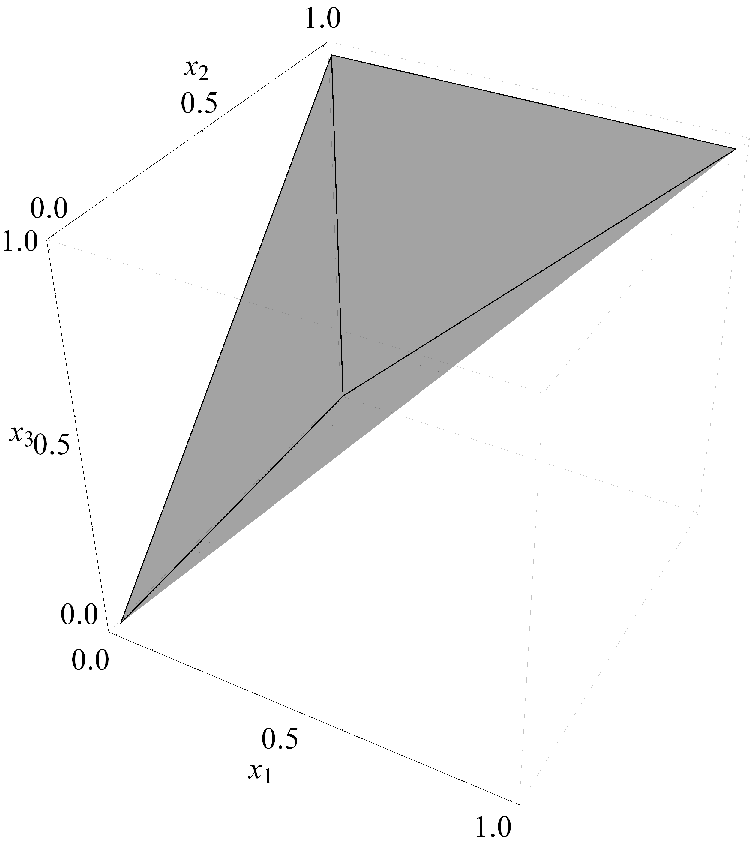
\includegraphics[width=2.5in]{ex1}\\
  \caption{Convex hull $conv(K)$}\label{Fig:Example1}
\end{figure}
We have $3! = 6$ permutations and corresponding extended polymatroid inequalities. We tabulate the coefficient pertaining to these inequalities in Table \ref{tab:example}
\begin{table}[htbp]
  \centering
  \caption{Tabulating polymatroid coefficients for different permutations}
    \begin{tabular}{c|ccc|ccc}
    \toprule
    $\bpi = \{(1),(2),(3)\}$ & $f(\{(1)\})$ & $f(\{(1),(2)\})$ & $f(N)$ & $v_1$   & $v_2$   & $v_3$ \\
    \midrule
    \{1,2,3\} & 2     & 2     & -2    & 2     & 0     & -4 \\
    \{1,3,2\} & 2     & 2     & -2    & 2     & 0     & -4 \\
    \{2,1,3\} & 1     & 2     & -2    & 1     & 1     & -4 \\
    \{2,3,1\} & 1     & -1    & -2    & 1     & -2    & -1 \\
    \{3,1,2\} & 2     & 2     & -2    & 2     & 0     & -4 \\
    \{3,2,1\} & 2     & -1    & -2    & 2     & -3    & -1 \\
    \bottomrule
    \end{tabular}%
  \label{tab:example}%
\end{table}%
In the first case, the natural permutation \{1, 2, 3\} yields $S = \{1,2\}$ and $C^+_{\bpi} = \{1\}$, $J_{\bpi} = \{3\}$, $C^-_{\bpi} = \emptyset$. Proposition \ref{prop:submodcover} yields the corresponding inequality,
\begin{align}
    x_1 \leq x_3 \label{ineq:exfacet1}
\end{align}

The remaining aforementioned permutations yield the following submodular cover inequalities,
\begin{align}
    x_1 &\leq x_2 \\
    x_1 + x_2 &\leq x_3 + 1 \\
    x_3 &\leq x_2 \label{ineq:exfacet2}\\
    x_3 &\leq x_1 + x_2\label{ineq:exampleend}
\end{align}
All of the aforementioned inequalities \eqref{ineq:exfacet1}-\eqref{ineq:exampleend} are valid for $\conv{K}$. Furthermore, inequalities \eqref{ineq:exfacet1} and \eqref{ineq:exfacet2} define the facets of $\conv{K}$.
\end{example}

\subsubsection{Pack Inequalities}
\label{sec:submodpack}
\hfill

 As per the preliminaries defined in Section \ref{sec:submodcover}, we define the notion of \textit{submodular packs} and characterize \textit{maximal submodular packs} as follows,
\begin{dfn}
  We define $S\subseteq N$, $S \define \{(1), (2), \ldots, (|S|)\}$ for some permutation $\bpi = \{(1), (2), (3),\ldots, |N|\}$ as a \emph{submodular pack} if $f(S) < b$. The corresponding residual capacity is $\delta \define b - f(S) > 0$.
\end{dfn}

\begin{prop}
  Consider $S\subseteq N$, $S \define \{(1), (2), \ldots, (|S|)\}$ for some permutation of $\bpi = \{(1), (2), (3),\ldots, |N|\}$, then $S$ is a submodular pack if and only if $S$ is an extended polymatroid pack.
\end{prop}
\begin{proof}
  The proof follows from the definitions.
  Let $S$ be an extended polymatroid pack, thus,
  \begin{align*}
    b & > \bv(S) = \sum_{i\in S} v^{\bpi}_{i}\\
      & = \sum_{(i)\in S} f(\{S^{\bpi}_i\}) - f(\{S^{\bpi}_{i-1}\})\\
      & = f(S) - f(\emptyset)\\
      & = f(S)
  \end{align*}
  Conversely, let $S$ be a submodular cover, i.e.
  \begin{align*}
    b & > f(S) = f(S) - f(\emptyset)\\
      & = f(S^{\bpi}_{|S|}) - \sum_{j = 1}^{|S|-1}(f(S^{\bpi}_{j}) - f(S^{\bpi}_{j})) - f(\emptyset)\\
      & = \sum_{j = 1}^{|S|}(f(S^{\bpi}_{j}) - f(S^{\bpi}_{j-1}))\\
      & = \sum_{j = 1}^{|S|} v^{\bpi}_j = \bv(S)
  \end{align*}
  The result follows.
\end{proof}

\begin{dfn}
We define $S\subseteq N$, $S \define \{(1), (2), \ldots, (|S|)\}$ for some permutation $\bpi = \{(1), (2), (3),\ldots, |N|\}$ as a \emph{maximal submodular pack with respect to $\bpi$} if,
  \begin{align*}
    & f(S\cup (j)) > b,\,\,\forall\,(j) \inset I_{\bpi}\sm S \text{   and },\\
    & f(S\,\sm\, (i)) > b,\,\,\forall\,(i) \inset J_{\bpi} \cap S
  \end{align*}
\end{dfn}

\begin{prop}
  Consider $S\subseteq N$, $S \define \{(1), (2), \ldots, (|S|)\}$ for some permutation of $\bpi = \{(1), (2), (3),\ldots, |N|\}$, then $S$ is a maximal submodular pack if $S$ is a maximal extended polymatroid pack {\revise{with respect to $\bpi$}}.
\end{prop}
\begin{proof}
  Notice that, for $S$ to be a maximal submodular pack with respect to $\bpi$,
  \begin{align*}
    & f(S\cup (j)) > b,\,\,\forall\,(j) \inset I_{\bpi}\sm S \text{   and },\\
    & f(S\,\sm\, (i)) > b,\,\,\forall\,(i) \inset J_{\bpi} \cap S
  \end{align*}
  In other words,
  \begin{align*}
     \rho_j(S) & > \delta,\,\,\forall\,(j) \inset I_{\bpi}\sm S \text{   and },\\
     -\rho_j(S\sm j) & > \delta,\,\,\forall\,(i) \inset J_{\bpi} \cap S
  \end{align*}

  If $S$ is a  maximal extended polymatroid pack with respect to $\bpi$ then,
  \begin{align*}
    v^{\bpi}_j  > \delta,\,\,\forall\,(j) \inset I_{\bpi}\sm S\,\,\text{ and } & -v^{\bpi}_j > \delta,\,\,\forall\,(j) \inset J_{\bpi} \cap S
  \end{align*}
  Since, $f$ is submodular, the difference function $\rho(\cdot)$ is a non-increasing function, which yields,
  $$
        v^{\bpi}_{(j)} \leq  \rho_{(j)}(S),\,\,\forall\,(j) \inset I_{\bpi}\sm S\,\,\text{ and }  v^{\bpi}_{(j)} \geq \rho_{(j)}(S\sm (j)),\,\,\forall\,(j) \inset J_{\bpi} \cap S
  $$
  thus we have,
  \begin{align*}
    \rho_j(S) > \delta,\,\,\forall\,(j) \inset I_{\bpi}\sm S \text{   and } -\rho_j(S\sm j) > \delta,\,\,\forall\,(i) \inset J_{\bpi} \cap S.
  \end{align*}
  The result follows.
\end{proof}

Define the sets $M^+_{\bpi}$ and $M^-_{\bpi}$ as follows,
\begin{align}
  M^+_{\bpi} & \define \set{(i)\in I_{\bpi}\sm S}{\rho_{(i)}(N\sm (i)) > \delta}\\
  M^-_{\bpi} & \define \set{(j)\in J_{\bpi}\cap S}{-\rho_{(j)}(\emptyset) > \delta}
\end{align}

\begin{prop}
    Consider $S\subseteq N$, $S \define \{(1), (2), \ldots, (|S|)\}$ for some permutation of $\bpi = \{(1), (2), (3),\ldots, |N|\}$. If $S$ is a submodular pack then the \emph{submodular pack inequality} with respect to $\bpi$,
    \begin{align}
      \sum_{(j) \in M^-_{\bpi}} x_{(j)} - \sum_{(i) \in M^+_{\bpi}} x_{(i)} \geq |M^-_{\bpi}| \label{ineq:submodpack}
    \end{align}
    is valid for $K^f_{S}$.
\end{prop}
%In addition, $S$ is a \emph{maximal submodular pack} if,
%  \begin{align*}
%    & f(S\cup (j)) > b,\,\,\forall\,(j) \inset I_{\bpi}\sm P^+ \text{   and },\\
%    & f(S\,\sm\, (i)) > b,\,\,\forall\,(i) \inset P^-
%  \end{align*}
%  where $P^+ \define I_{\bpi} \cap S$ and $P^- \define J_{\bpi} \cap S$
%\begin{prop}
%  Consider $S\subseteq N$, $S \define \{(1), (2), \ldots, (|S|)\}$ for some permutation of $\bpi = \{(1), (2), (3),\ldots, |N|\}$, then $S$ is a maximal extended polymatroid pack if $S$ is a maximal submodular pack.
%\end{prop}
%\begin{proof}
%  Notice that, for $S$ to be a maximal extended polymatroid cover,
%  \begin{align*}
%     |v_j| & > \lambda,\,\,\forall\,\,j\in N\sm {P^+ \cup P^-}
%  \end{align*}
%
%  If $S$ is a maximal submodular cover then,
%  \begin{align*}
%    \rho_{(j)}(S)  > \delta,\,\,\forall\,(j) \inset I_{\bpi}\sm P^+ \text{   and }
%    -\rho_{(j)}(S\,\sm\, (j)) > \delta,\,\,\forall\,(i) \inset P^-
%  \end{align*}
%  Since, $f$ is submodular, the difference function $\rho(\cdot)$ is a non-increasing function, which yields,
%  $$
%        v^{\bpi}_{(j)} \leq  \rho_{(j)}(S),\,\,\forall\,(j) \inset I_{\bpi}\sm P^+ \text{   and }  v^{\bpi}_{(j)} \geq \rho_{(j)}(S\sm (j)),\,\,\forall\,(j) \inset C^+_{\bpi}
%  $$
%  thus we have,
%  \begin{align*}
%    -v^{\bpi}_{(j)}  > \lambda,\,\,\forall\,(j) \inset J_{\bpi}\sm C^-_{\bpi}\,\,\text{ and } & v^{\bpi}_{(j)} > \lambda,\,\,\forall\,(j) \inset C^+_{\bpi}
%  \end{align*}
%  The result follows.
%\end{proof}

Submodular pack inequalities \eqref{ineq:submodpack} are derived from the restrictions of the submodular knapsack polytope and are valid for the corresponding projections and not necessarily for $K^f$. Weight inequalities \cite{Weismantel97} as seen in Sections \ref{sec:pack} and \ref{sec:genpack} that are valid for the knapsack set, can be directly generalized to the case of submodular knapsack \textit{via} extended polymatroid associated with the corresponding set function $f$. We formalize this in the following result.

\begin{prop}
  The submodular weight inequality,
  \begin{align}
    \sum_{j\in J_{\bpi}\sm S} \rho_{j}(N\sm j)x_j - \sum_{i \in S\cap I_{\bpi}} f(i)(1-x_i) + \sum_{i \in I_{\bpi}\sm S} (\rho_{i}(N\sm i) - \delta)^+x_i + \sum_{j \in S\cap J_{\bpi}} (-f(j) - \delta)^+ (1-x_j) \leq 0
  \end{align}

  is valid for $K_f$.
\end{prop}
\begin{proof}
  Consider a permutation $\bpi = \{1,2,\ldots,n\}$ of the elements of the index set $N$. Define the corresponding index sets $I_{\bpi}$ and . Proposition \ref{prop:genweight} suggests that the following weight inequality,
  \begin{align*}
     \sum_{j \in J_{\bpi}\sm S} v^{\bpi}_j x_j - \sum_{i\in  S\cap I_{\bpi}} v^{\bpi}_i(1-x_i) + \sum_{i \in  I_{\bpi}\sm S} (v^{\bpi}_i - \bar{\delta})^+ x_i + \sum_{j \in S\cap J_{\bpi}} (-v^{\bpi}_j - \bar{\delta})^+ (1-x_j) \leq 0
  \end{align*}
is valid for $K_f$.  Furthemore, submodularity of the set function $f$ suggests,
\begin{align*}
	 \rho_{j}(N\sm j) \leq v^{\bpi}_j \leq f(j),\, & \forall \,\, j \in  N,\,\, \forall \,\,\bpi
\end{align*}
The result follows.
\end{proof}
\begin{example}
\tba
\end{example}
\subsection{Strengthening the valid inequalities \textit{via} Extensions}\hfill

As in the case of linear $0-1$ knapsack, we can strengthen the inequalities corresponding to \textit{submodular covers} \eqref{ineq:submodcover} and \textit{submodular packs} \eqref{ineq:submodpack} via computationally efficient extensions. In the following discussion we provide an analogous procedure to extend these inequalities as in Section \ref{sec:extension}.

Consider the subset $S \subseteq N$ as earlier in Section \ref{ineq:submodcover}. Before we generalize the extensions for submodular set functions, we would like to define a few preliminaries.
\begin{dfn}
  Reconsider the permutation $\bpi$, and the corresponding complement set $\bpi^{(N\sm S)} = \{(|S|+1),(|S|+2)\ldots,(|N|)\}$ and let $S_k = S \cup \{(|S|+1), (|S|+2), \ldots, (|S|+k)\},\,\,\forall\,k = 1,2,\ldots,|N\sm S|$. We define the extension of $C^+_{\bpi} \subseteq S$ and reduction of $C^-_{\bpi} \subseteq S$ with respect to $\bpi^{(N\sm S)}$ as $E_{\bpi}^+ \define (I_{\bpi}\sm C^+_{\bpi}) \cap E$ and $R_{\bpi}^- \define C^-_{\bpi} \cap E$ respectively, where,
  \begin{align*}
    & E \define \set{(i) \in (I_{\bpi}\sm C^+_{\bpi}) \cup C^-_{\bpi}}{|v^{\bpi}_{(i)}| > \underset{(j) \in (C^+_{\bpi} \cup J_{\bpi}\sm C^-_{\bpi})}{\max}\{f(j),f(N\sm (j)) - f(N)\} - \lambda}
  \end{align*}
  Alternatively,
  \begin{align*}
    & E \define \set{(k) \in (I_{\bpi}\sm C^+_{\bpi}) \cup C^-_{\bpi}}{|\rho_{(k)}(S_{k-1})| > \underset{(j) \in (C^+_{\bpi} \cup J_{\bpi}\sm C^-_{\bpi})}{\max}\{f(j),|\rho_{(j)}(N\sm (j))|\} - \lambda}
  \end{align*}
  %where $\lambda_k \define \lambda_{k-1} - \left(\underset{(j) \in (C^+_{\bpi} \cup J_{\bpi}\sm C^-_{\bpi})}{\max}\{f(j),|\rho_{(j)}(N\sm (j))|\} - |\rho_{(k)}(S_{k-1})|\right)^+$\\
  where $\lambda = f(S) - b$
\end{dfn}

Owing to the above preliminaries, we now present the following result leading to the extensions of submodular cover inequalities \eqref{ineq:submodcover} which is a direct generalization of Proposition \ref{prop:genextcover}.

\begin{prop}
  If $f(S) > b$, the extended submodular cover inequality,
  \begin{align}
  \label{ineq:submodextcover}
    \x(\bar{C}^+_{\bpi}) - \x(J_{\bpi}\sm\bar{C}^-_{\bpi}) \leq |C^+_{\bpi}| - (|{C}^-_{\bpi}\sm \bar{C}^-_{\bpi}| + 1)
  \end{align}
  where $\bar{C}^+_{\bpi} = C^+_{\bpi} \cup E_{\bpi}^+$ and $\bar{C}^-_{\bpi} = C^-_{\bpi} \sm R_{\bpi}^-$, is valid for $\conv(K^f)$. Additionally, inequality \eqref{ineq:submodextcover} defines a facet of $\conv(K^f_{\bar{C}^+_{\bpi}\cup J_{\bpi}\sm\bar{C}^-_{\bpi}})$ if and only if $S$ is maximal with $C^+_{\bpi}$ minimal and if $\forall$ $(i) \inset E_{\bpi}^+ \cup R_{\bpi}^-$ $\exists$ distinct $\{(j),(k)\} \inset S$ such that $$f(S\cup (i)\sm \{(j),(k)\})\leq b$$
\end{prop}

\begin{rem}
  It should be observed that as in the case of $0-1$ linear knapsack, and stated in Proposition \ref{prop:genextcover}, the extensions for submodular knapsack are \emph{not} sequence independent.
\end{rem}

\begin{rem}
  In the special case when $J_{\bpi} = \emptyset,\, \forall\, \bpi$ i.e. $f$ is non decreasing on $N$, inequality \eqref{ineq:submodextcover} yields an extension for the case considered in \cite{Atamturk2009333}. Though their result of Proposition 5 \cite{Atamturk2009333} is derived directly from the subadditive lower bound $\varphi(a)$ for lifting function $\Theta(a)$ \cite{Atamturk2005}.
\end{rem}

\begin{dfn}
  Reconsider the permutation $\bpi$, and the corresponding complement set $\bpi^{(N\sm S)} = \{(|S|+1),(|S|+2)\ldots,(|N|)\}$ and let $S_k = S \cup \{(|S|+1), (|S|+2), \ldots, (|S|+k)\},\,\,\forall\,k = 1,2,\ldots,|N\sm S|$. We define the extension of $M^+_{\bpi} \subseteq N\sm S$ and $M^-_{\bpi} \subseteq N \sm S$ with respect to $\bpi^{(N\sm S)}$ as $E_{\bpi}^+ \define (I_{\bpi}\sm C^+_{\bpi}) \cap E$ and $R_{\bpi}^- \define C^-_{\bpi} \cap E$ respectively, where,
  \begin{align*}
    & E \define \set{(i) \in (N\sm (M^+_{\bpi} \cup M^-_{\bpi}))}{|v^{\bpi}_{(i)}| + \delta > \underset{(j) \in (M^+_{\bpi} \cup M^-_{\bpi})}{\max}\{f(j),f(N\sm (j)) - f(N)\}}
  \end{align*}
  Alternatively,
  \begin{align*}
    & E \define \set{(k) \in (I_{\bpi}\sm C^+_{\bpi}) \cup C^-_{\bpi}}{|\rho_{(k)}(S_{k-1})| > \underset{(j) \in (C^+_{\bpi} \cup J_{\bpi}\sm C^-_{\bpi})}{\max}\{f(j),|\rho_{(i)}(N\sm (i))|\} - \lambda}
  \end{align*}
  %where $\lambda_k \define \lambda_{k-1} - \left(\underset{(j) \in (C^+_{\bpi} \cup J_{\bpi}\sm C^-_{\bpi})}{\max}\{f(j),|\rho_{(i)}(N\sm (i))|\} - |\rho_{(k)}(S_{k-1})|\right)^+$\\
  where $\lambda = f(S) - b$
\end{dfn}


\subsection{Lifted Submodular Cover Inequalities}\hfill
\label{sec:submodlifting}

In this section we study the lifting problem of the valid inequalities discussed earlier in order to strengthen them. The lifting procedure has been very effective in strengthening inequalities for the linear $0-1$ min-knapsack set \cite{Balas1975,Balas1978,Balas1984,Gu1998,Hammer1975,Wolsey1975} as described in Section \ref{sec:extension}.

\subsubsection{Cover Inequalities}\hfill

The lifting problem for the submodular cover inequalities for $K_f$ is itself an optimization problem over the supermodular knapsack set.

In particular, we lift the submodular cover inequality \eqref{ineq:submodcover} to a valid inequality of the form,
\begin{align}
  \label{ineq:liftedsubmodcover}
  \x(C^+_{\bpi})  - \x(J_{\bpi}\sm C^-_{\bpi}) + \sum_{i\,\in I_{\bpi}\sm C^+_{\bpi}} \alpha_i x_i - \sum_{j\,\in C^-_{\bpi}} \alpha_j x_j \leq |C^+_{\bpi}| - (\boldsymbol\alpha(C^-_{\bpi}) + 1)
\end{align}
where $\alpha_i \in \R,\, i \in ( C^-_{\bpi} \cup I_{\bpi}\sm C^+_{\bpi})$ are the corresponding lifting coefficients. Observe that, $\alpha_i \geq 0,\, i \in I^+\sm C^+_{\bpi}$ and $\alpha_j \geq 0,\, j \in I^-\cap C^-_{\bpi}$

\subsection{Sequence Independent Bounds on Lifting Coefficients}\hfill
\label{sec:submodseqind}

Akin to the linear $0-1$ knapsacks, we can derive the sequence independent lifting coefficients for the submodular knapsack $K_f$. It is now that we will utilize the results from Section \ref{sec:gencover} to derive these bounds. In addition we will also demonstrate that the earlier results by \atam and Narayanan \cite{Atamturk2009333} are a special case of these generalizations. Before proceeding, we define the following preliminaries,

\begin{dfn}
  For an index set $T$, and a permutation $\bpi = \{(1),(2),\ldots, (|T|)\} \in \Pi_T$ the set of all permutations of elements of $T$, we define the set function $\bar{f}\,:\,\binset^{|T|} \mapsto \R$ as,
  \begin{align}
    \bar{f}(\bpi) = \sum_{i\in 1}^{|T|} |\rho_{(i)}(T_{i-1})|
  \end{align}
  where $T_k = \{(1), (2), \ldots, (k)\},\,\,\forall\,k = 1,2,\ldots,|T|$ and $T_0 = \emptyset$.
\end{dfn}
Observe that when $f$ is monotone non-decreasing (non-increasing) then $\bar{f}(\bpi)$ is independent of the permutation $\bpi \in \Pi_T$ and evaluates to $f(T)$ ($-f(T)$).

\begin{dfn}
 For an index set $T$, and a permutation $\bpi = \{(1),(2),\ldots, (|T|)\} \in \Pi_T$ the set of all permutations of elements of $T$, we define
  \begin{align}
         A_h & \define {\max}\,\,\set{\bar{f}(\bpi)}{T\subseteq C^+_{\bpi} \cup (J_{\bpi}\sm C^-_{\bpi}),\,\,|T| = h,\,\,\bpi \in \Pi_T}.\\ %\underset{\substack{T\subseteq C^+_{\bpi} \cup C^-_{\bpi}\\|T| = h\\ \bpi \in \Pi_T}}
         B_h & \define {\min}\,\,\set{\bar{f}(\bpi)}{T\subseteq C^+_{\bpi} \cup (J_{\bpi}\sm C^-_{\bpi}),\,\,|T| = h,\,\,\bpi \in \Pi_T}. %\underset{\substack{T\subseteq C^+_{\bpi} \cup C^-_{\bpi}\\|T| = h\\ \bpi \in \Pi_T}}
  \end{align}
\end{dfn}

\begin{prop}
  For $k\in (C^-_{\bpi} \cup I_{\bpi}\sm C^+_{\bpi}),$ $\alpha_k \geq h,$ if
  \begin{align}
    \min\{|f(k)|,|\rho_{i}(N\sm i)|\} \geq A_h
  \end{align}
\end{prop}

\begin{prop}
  For $k\in (C^-_{\bpi} \cup I_{\bpi}\sm C^+_{\bpi}),$ $\alpha_k \leq h,$ if
  \begin{align}
    \max\{|f(k)|,|\rho_{i}(N\sm i)|\} \leq b + \underset{\bpi \in \Pi_{J_{\bpi}}}{\min}\bar{f}(\bpi) - B_{|C^+_{\bpi} \cup (J_{\bpi}\sm C^-_{\bpi})|-1-h}
  \end{align}
\end{prop}

\begin{rem}
  In the special case when $J_{\bpi} = \emptyset,\, \forall\, \bpi$ i.e. $f$ is non decreasing on $N$, inequality \eqref{ineq:submodextcover} yields the result of Proposition $7$ on sequence independent lifting coefficients \cite{Atamturk2009333}.
\end{rem}
\bibliographystyle{plain}
\bibliography{SubmodPolymatroid}
\end{document} 